\chapter{绪论}
相变是凝聚态物理学的核心内容之一,其描述了系统在外部参数变化时从一种物理相向另一种相的突变。
朗道相变理论(Landau Phase Transition Theory)是由苏联物理学家朗道(Lev Landau)提出的一种描述相变的唯象理论\cite{landau1937theory,landau1980statistical}。
在朗道相变理论中,相变是序参量及其导数和高阶导数的不连续行为。
这种不连续性,是系统对称性破缺的结果。
朗道相变理论通过对称性破缺和自由能的极小化原理,系统地解释了相变机制。
尽管朗道相变理论成功地描述了广泛的相变现象,但它本质上局限于对称性破缺驱动的相变。
随着对量子材料理解的深入,朗道相变理论的局限性逐渐显现,促使拓扑相变等新概念的提出。

拓扑相变是一类不同寻常的相变,其特征不是对称性破缺或局部序参量,而是全局拓扑不变量的变化。
1980年,冯·克利青(Klaus von Klitzing)在实验中发现了整数量子霍尔效应(Integer quantum hall effect, IQHE)\cite{klitzing1980new}。
这一效应揭示了系统的电导值由一个整数(拓扑不变量,即Chern数)决定,与传统的对称性破缺理论无关。
1982年,David J. Thouless及其合作者(Kohmoto, Nightingale, and den Nijs)通过TKNN理论从拓扑数学的角度
解释了量子霍尔效应\cite{thouless1982quantized},首次将拓扑不变量引入凝聚态物理。
与传统相变不同,拓扑相变起源于系统波函数拓扑性质的变化,为相变行为提供了一种全新的视角。

1982年, 华人物理学家崔琦, 德国物理学家 Stormer发现横向电阻不仅可以取正整数, 还出现了 n=1/3 这样一个分数的平台\cite{tsui1982two},
标志着分数量子霍尔效应(Fractional quantum hall effect)的发现。
1983年,劳克林(Laughlin)通过构造分数量子霍尔态的波函数成功解释了这一现象\cite{laughlin1983anomalous},首次提出了拓扑序(Topological order)的概念。不同于传统的能带拓扑,分数量子霍尔效应是一种拓扑序现象,其起源于粒子之间的纠缠性质。拓扑序将拓扑相的概念扩展到超越能带理论的领域,涵盖具有长程量子纠缠的物质相。与对称性破缺相不同,拓扑序的特征是依赖于空间拓扑的基态简并性以及具有分数统计的奇异准粒子。拓扑序为量子物质提供了更深层的理解,并因其拓扑态对局部扰动的鲁棒性而在容错量子计算中具有潜在应用。

本章主要介绍了拓扑相变的基本概念和基本原理,介绍量子霍尔效应,反常量子霍尔效应,分数量子霍尔效应以及高阶拓扑绝缘体(High-order topological insulator,HOTI)等经典拓扑模型的发展脉络,以及其相应的拓扑不变量以及物理特性。
\section{拓扑绝缘体}
拓扑学是数学的一个分支,涉及在连续变形下保持的量。在拓扑学中,封闭的表面可以平滑地变形为各种几何形状,而无需剪切和粘贴。例如,图 \ref{fig:TopoGeo} 中的 6 个对象都有不同的几何结构,但只有三种不同的拓扑结构。球体可以不断变为勺子,因此它们在拓扑上是等效的。
圆环和咖啡杯在拓扑上也是等价的,双圆环和茶壶也是如此。这些不同几何的拓扑可以用Gauss-Bonnet定理描述,
\begin{equation}
	\frac{1}{2\pi}\int_{surface}KdA=2(1-g)
\end{equation}
它指出二维闭合表面的总高斯曲率 (K) 始终是一个整数。这个拓扑不变量称为亏格 (g),描述了表面的拓扑结构,即内部的孔数。拓扑不变量在系统的连续变形下保持不变。具有相同拓扑不变量的对象在拓扑上是等效的;也就是说,它们处于相同的拓扑阶段。只有在对象中创建或删除孔时,拓扑不变量才会更改。这个过程被称为拓扑相变。

\begin{figure}[htbp]
	\centering
	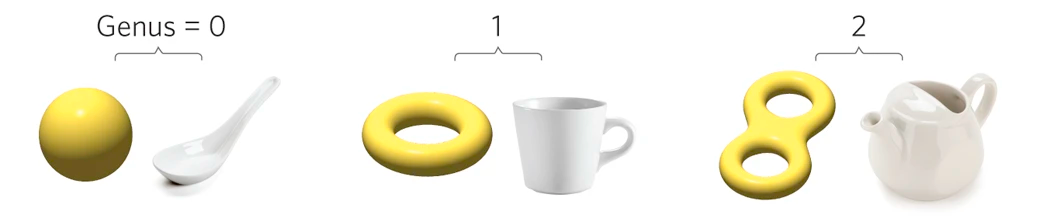
\includegraphics[width=0.75\textwidth]{figure/Introduction/TopoGeo.png}
 \caption{拓扑等价性示意图。可以将 6 个不同几何图形的对象分组为三对拓扑。每对都有相同的拓扑不变量,称为其亏格。图片来源于文献\cite{lu2014topological}。}
 \label{fig:TopoGeo}
\end{figure}

拓扑绝缘体的拓扑结构则定义在倒易(波矢)空间的能带上。二维布里渊区(Brillouin zone)也是一个封闭表面,由于其周期性边界条件,它与环面具有相同的拓扑结构。二维能带最经典的拓扑不变量是陈数(Chern number),其用于表征波段上波函数的Berry相位的拓扑结构。陈数是在圆环面上对 Berry 曲率的积分,它给出了二维表面的总量子化 Berry 通量的度量。在这个圆环面上Berry磁通会产生一些单极子,它们是是Berry相位的奇点,可以类比为几何的孔洞。
因此陈数本质上就是这些单极子的数目,类似于亏格在前述几何中的定义。此外,一旦物理可观测量可以写为类似的拓扑不变量,它就只会离散地改变。因此,它不会响应连续的小扰动,这代表这其具有拓扑鲁棒性。

拓扑绝缘体最迷人的现象出现在边界。如图\ref{fig:TopoBand}(a, b)所示,当界面两边的绝缘体具有相同的拓扑时,其沿着参数x连续变化不会有任何拓扑上的突变。因此它们可以之间跨越能隙相连,无需关闭能隙。
而当界面两边具有不同拓扑时,连续变化参数x会在界面处出现能带拓扑的突变。因此能带拓扑不会允许它们直接连接,必须在界面处闭合带隙以中和陈数。而在此处闭合能隙的就是边缘态。这些边缘态来源于界面两边不同的拓扑,因此它们是拓扑保护的。边缘态的数目等于界面两边陈数的差异,这被称为体边对应,如图\ref{fig:TopoBand}(c)所示。
\begin{figure}[htbp]
	\centering
	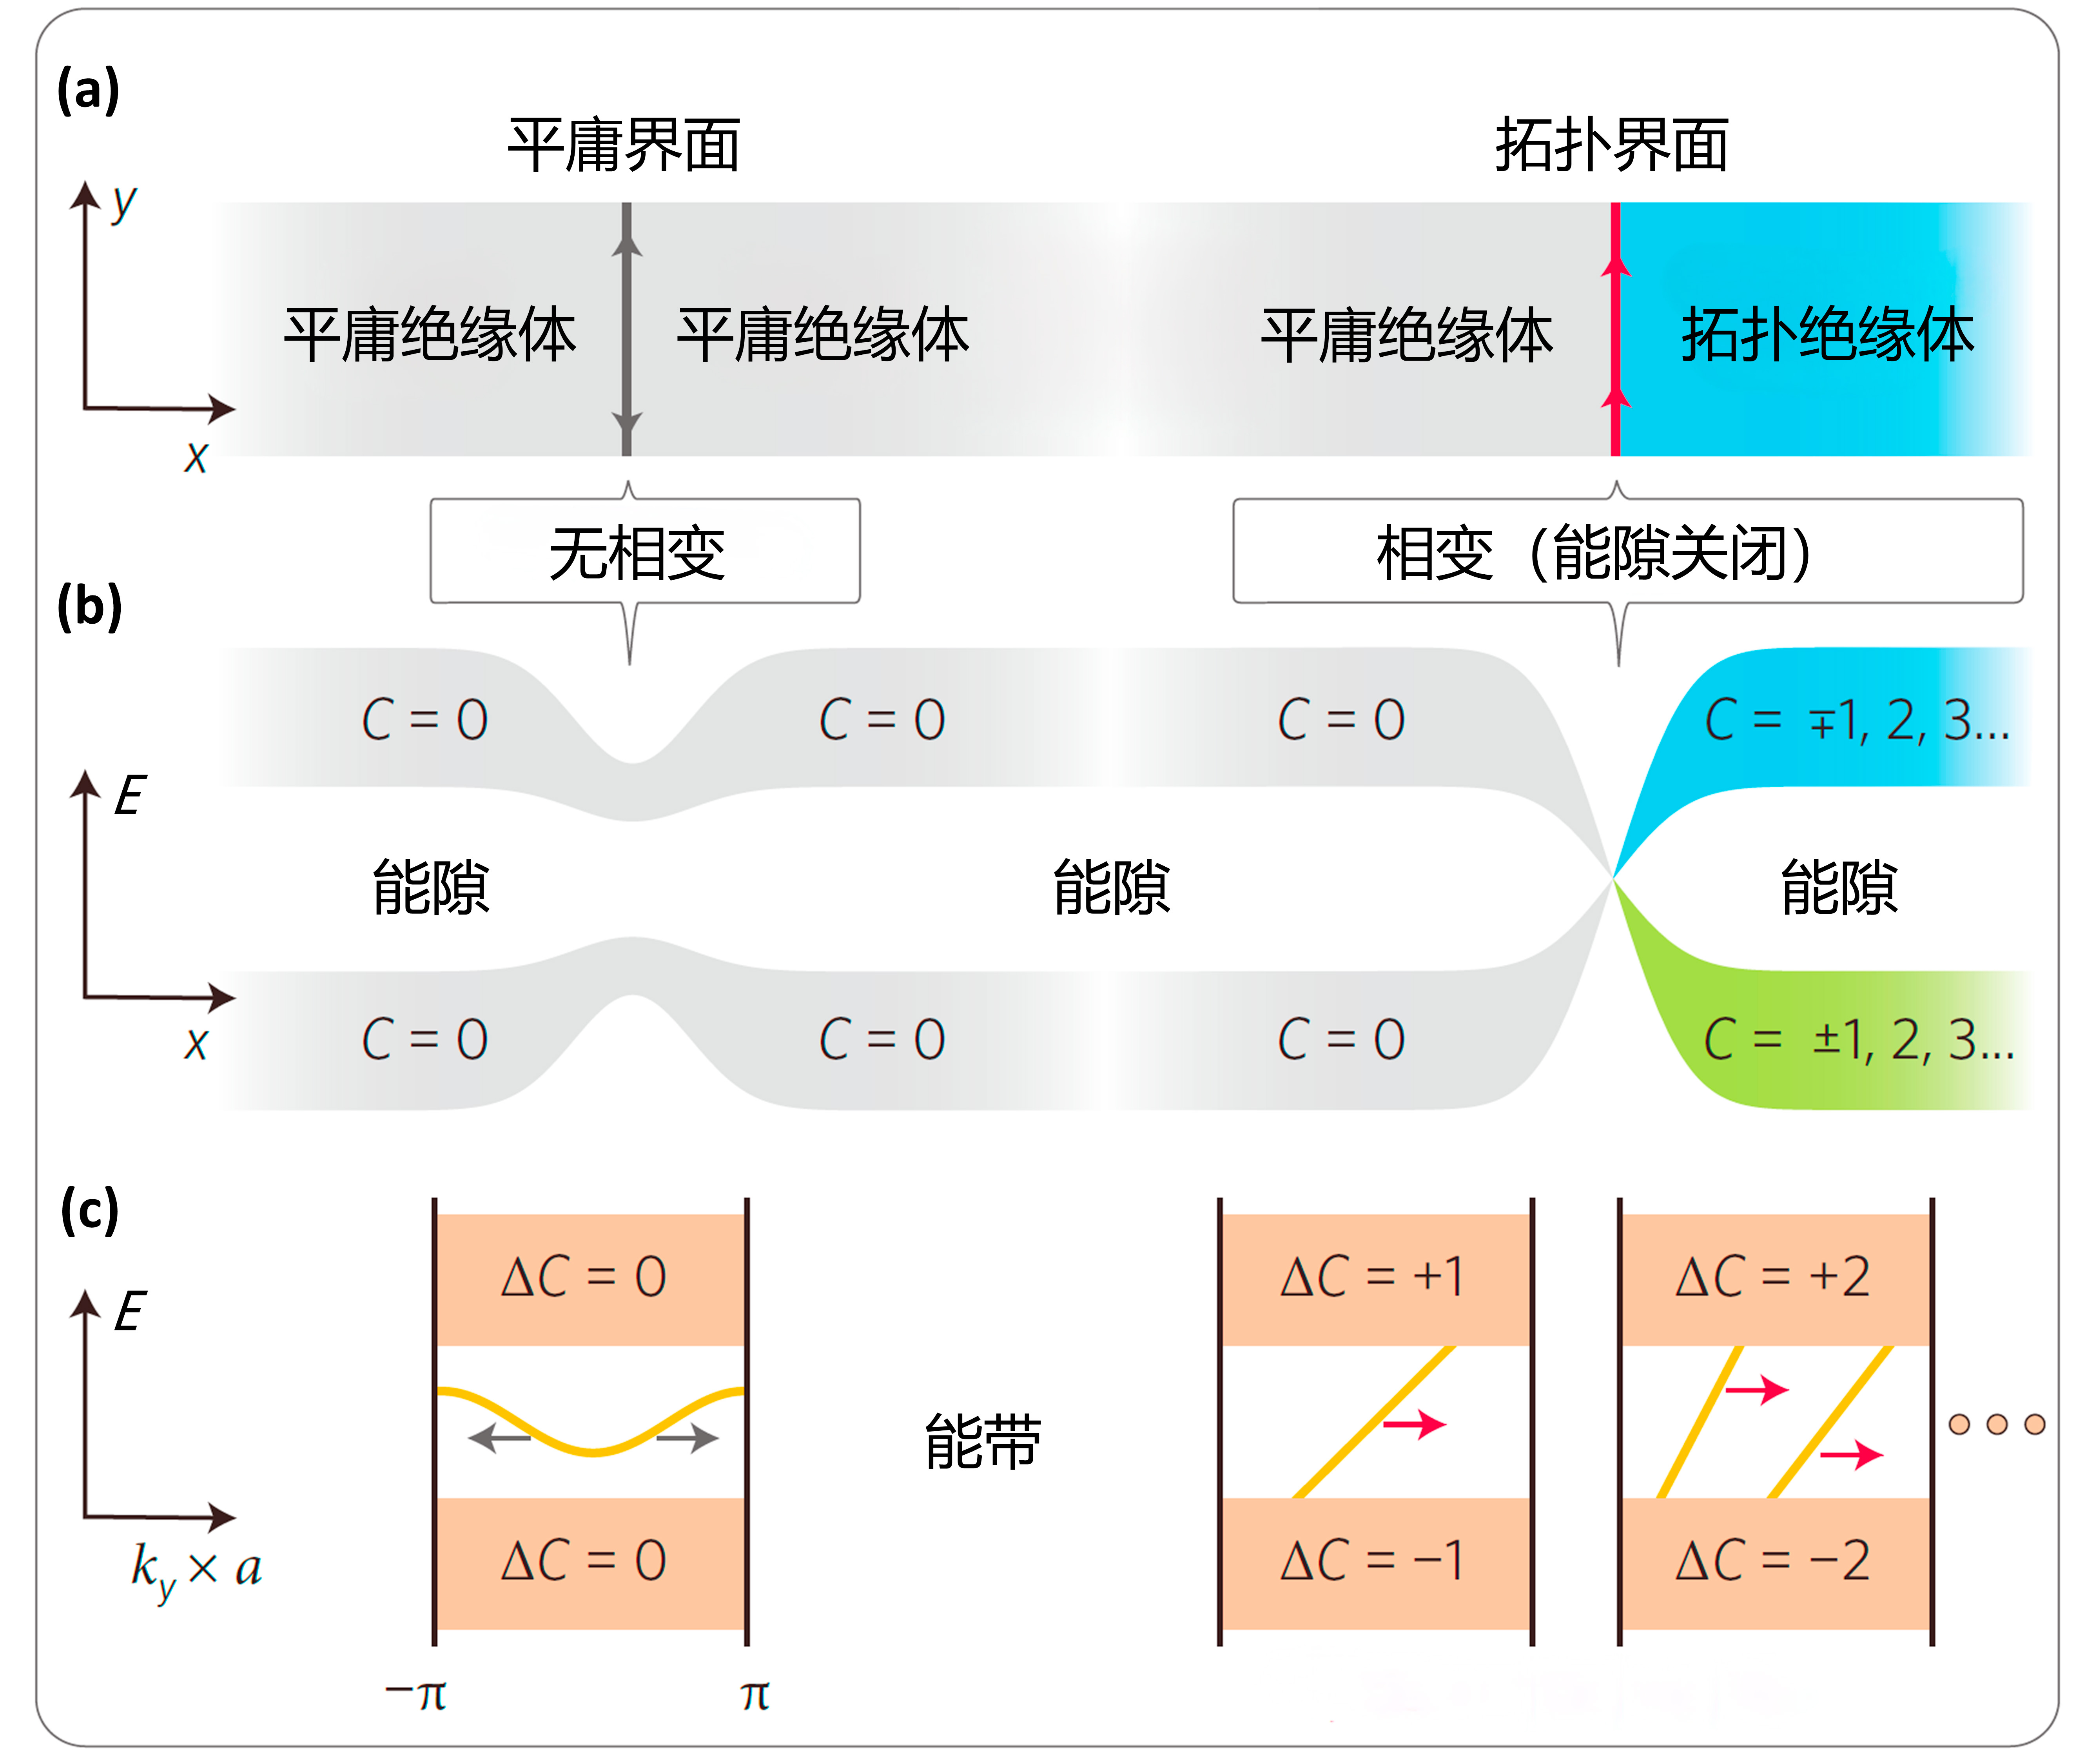
\includegraphics[width=0.75\textwidth]{figure/Introduction/TopoBand.jpg}
 \caption{能带拓扑示意图。(a) 由不同(右)和相同(左)拓扑的绝缘体形成的两个界面。
(b) 不同拓扑结构的频段如果不闭合带隙就无法相互过渡。
(c) 界面态与体带具有不同的连通性,具体取决于绝缘体内的能带拓扑。
 其中,a 是波导沿y方向传播的周期,$\Delta C$是波导右侧和左侧相应体带之间陈数的变化。
 $\Delta C$的大小等于无间隙界面模式的数量,$\Delta C$的符号表示传播方向。
图片来源于文献\cite{lu2014topological}。}

 \label{fig:TopoBand}
\end{figure}

\section{一阶拓扑绝缘体}
一阶拓扑绝缘体是最经典的拓扑绝缘体。其指的是在拓扑边界态与晶格的维度(余维度)相差一的拓扑绝缘体。譬如量子霍尔效应,其是二维材料产生一维的拓扑边界态;而若晶格为三维,则应产生二维的拓扑表面态。本节将介绍经典的一阶拓扑绝缘体,包括量子霍尔效应,反常量子霍尔效应,分数量子霍尔效应等模型。并探讨它们经典的理论实验工作,拓扑不变量,以及各自独特的拓扑现象。

\subsection{量子霍尔效应}
最经典的拓扑系统是整数量子霍尔效应,其描述了一个二维晶格在均匀z方向磁场下的情况。整数量子霍尔效应由冯·克利青(Klaus von Klitzing)由1980年在实验中观测到\cite{klitzing1980new},作者发现霍尔电导在低温下出现了量子化现象
\begin{equation}
	\sigma_{xy}=Ne^2/h
\end{equation}
其中,N是任意整数,e是电子电荷,h是普朗克常数。1982年,David J. Thouless及其合作者意识到这种独特的量子化现象来自于波函数的拓扑相变\cite{thouless1982quantized},首次将拓扑不变量引入凝聚态物理。

电子在磁场中的运动会受到磁场的影响,其可通过磁矢势的形式$\mathbf{B}=\nabla\times \mathbf{A}$描述。电子的动量$p$会受到矢量势的影响,从而变为广义动量:
\begin{equation}
	\mathbf{p}\to \mathbf{p}-\frac{e}{c}\mathbf{A}
\end{equation}
其中$e$是电子电荷,$c$是光速。在晶格系统的紧束缚模型中,电子在不同晶格点之间跃迁时,波函数会受到相位因子的修正,这被称为佩尔斯(Peierls)替换$J_{ij}\to J_{ij}e^{i\phi_{ij}}$。其中$J_{ij}$是跃迁振幅,而$\phi_{ij}=\frac{e}{\hbar c}\int_{r_i}^{r_j} A(r) \cdot dl$是电子从晶格点$i$到$j$积累的Aharonov-Bohm (AB) 相位。

\begin{figure}[htbp]
	\centering
	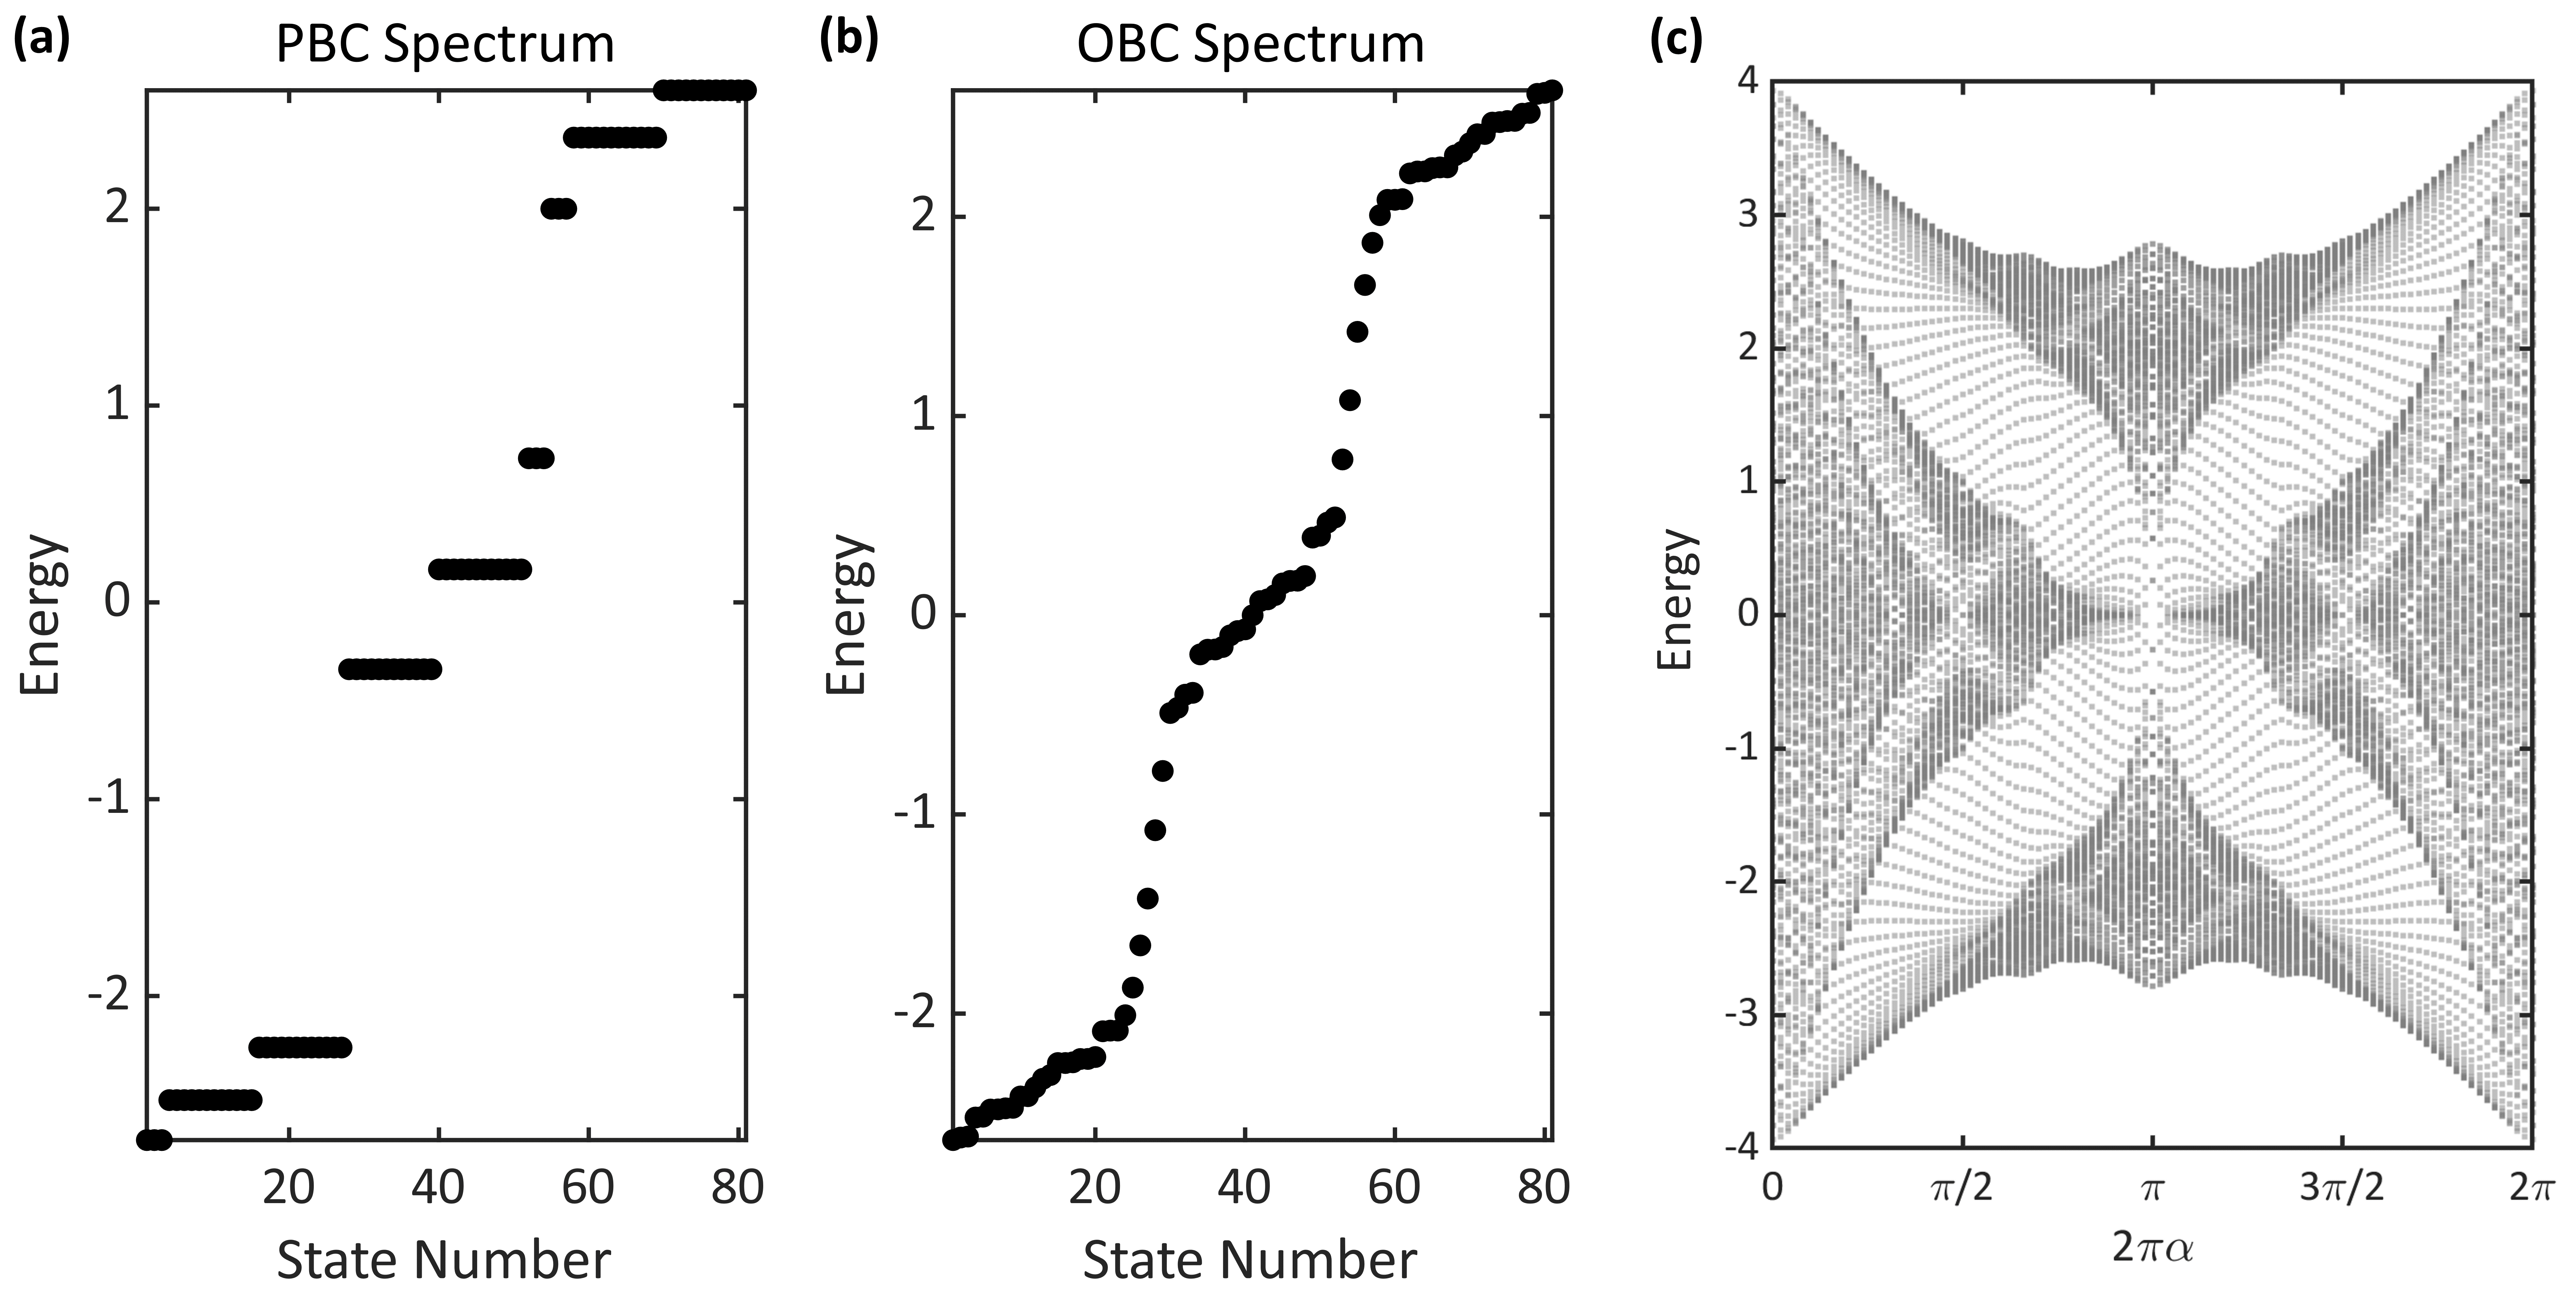
\includegraphics[width=0.9\textwidth]{figure/Introduction/Hofstadter.png}
 \caption{量子霍尔效应的能谱与霍夫斯塔特蝴蝶。(a) 周期性边界条件下的量子霍尔效应能谱图。晶格大小为$9\times9$,磁场选取为$\alpha=1/3$。
(b) 开放性边界条件下的量子霍尔效应能谱图。
(c) 方晶格的霍夫斯塔特蝴蝶。晶格大小为$16\times16$。}
 \label{fig:Hofstadter}
\end{figure}

本文以方晶格为例,选取朗道规范,磁场下哈密顿量的紧束缚形式可以写为,
\begin{equation}
	H=-J\left[\hat{a}_2^{\dagger} \hat{a}_1 e^{-i \phi_{12}}+\hat{a}_3^{\dagger} \hat{a}_2+\hat{a}_4^{\dagger} \hat{a}_3 e^{i \phi_{34}}+\hat{a}_1^{\dagger} \hat{a}_4\right]+\text { h.c. }
\end{equation}
其中J是耦合常数,$\phi_{12}$和$\phi_{34}$是耦合时的跃迁相位。格点间的相位导致电子沿原胞绕一圈会积累相位$\phi_{34}-\phi_{12}=2\pi\alpha$。因此在每个小方格,会产生$2\pi\alpha$的磁通。

对晶体引入匀强磁场后,每条能带会产生劈裂。此时系统的能谱变为一系列能级,在低能处的能级就是著名的朗道能级,如图\ref{fig:Hofstadter}(a)所示。当将晶格由周期性边界条件变为开放边界条件时,系统会在能级间产生边缘态,填满能隙,如图\ref{fig:Hofstadter}(b)所示。
而当我们调节磁场大小,劈裂的能级会形成著名的霍夫斯塔特蝴蝶 (Hofstadter butterfly)。其是朗道能级的高能形式,如图\ref{fig:Hofstadter}(c)所示。

在图\ref{fig:HallEdgeState}(a)中,为了更清晰的展示边缘态,我们取一边周期性边界,一边开放性边界的量子霍尔效应。如图所示,在体能隙内出现了交叉的边缘态。这些单调的边缘态表明其群速度$v_g=\frac{\partial E}{\partial k}$始终为正或负。可以发现在一个带隙中出现了两个相反的边缘态。这是由于我们截取开放边界时带来了两个边界,两个边界的边缘态相反传输。接下来我们利用实空间的动力学说明边缘态的单向性和鲁棒性。如图\ref{fig:HallEdgeState}(b, c)所示,我们利用点源激发(蓝色圆点)拓扑带隙中的能量,此时边缘态仅向逆时针方向传输,并且可以单向传输过晶格的角,不出现背向散射。

\begin{figure}[htbp]
	\centering
	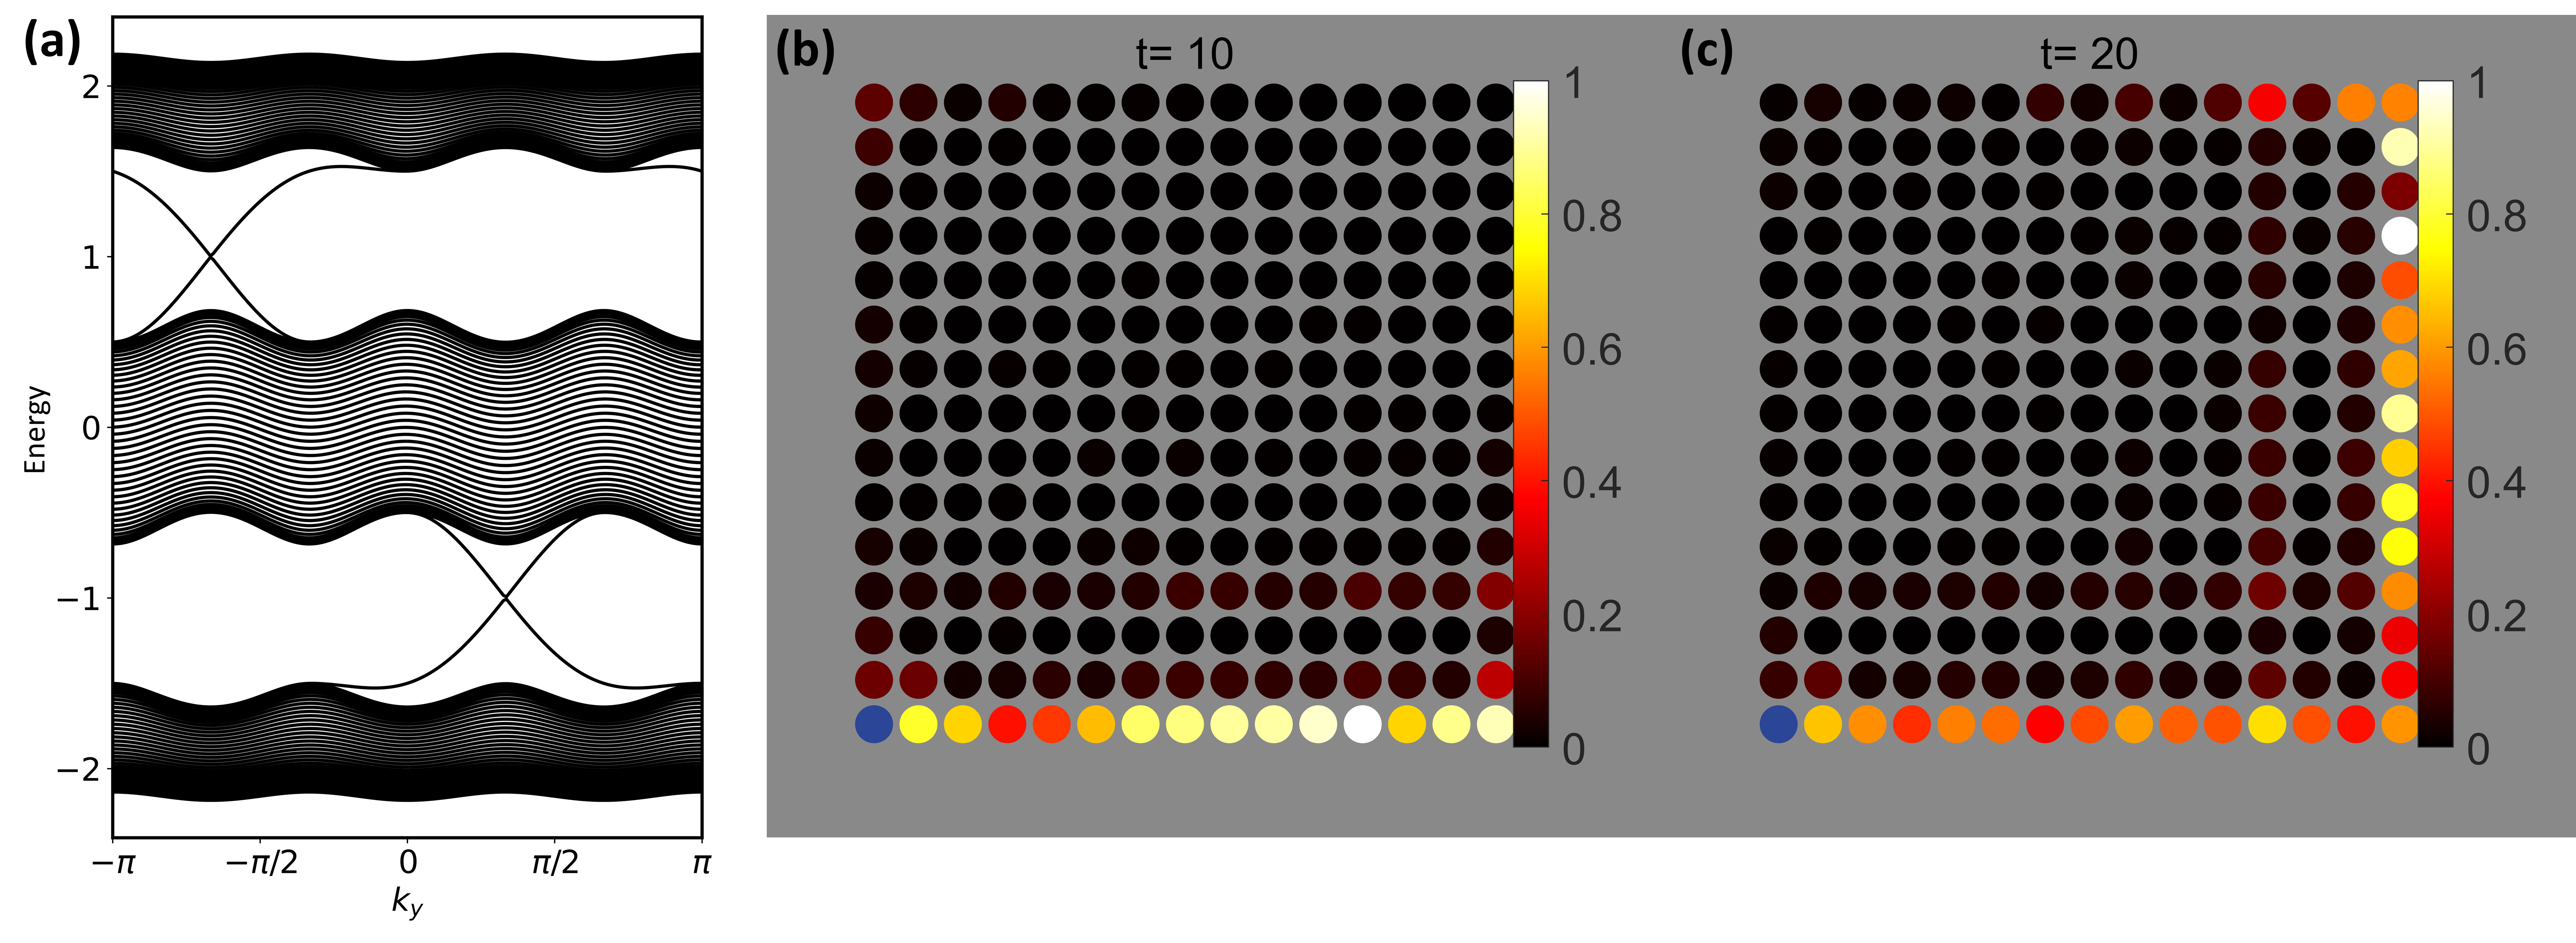
\includegraphics[width=1\textwidth]{figure/Introduction/HallEdgeState.png}
 \caption{量子霍尔效应的能谱与边缘态。(a) x方向周期性边界条件,y方向周期性边界条件的量子霍尔效应能谱图。x方向长度120,磁场选取为$\alpha=1/3$。
	(b, c) 在点源激发下的单向边缘态传输。晶格大小为$15\times15$。} 
 \label{fig:HallEdgeState}
\end{figure}

量子霍尔效应是凝聚态体系最经典的拓扑模型。整数量子霍尔效应的发现激发了对于拓扑绝缘体与拓扑相的研究。除了冯·克利青在凝聚态体系的经典实验\cite{klitzing1980new},量子霍尔效应也被理论和实验在光学\cite{Haldane2008prl,Haldane2008pra,ZhengWang2008prl,wang2009observation,hafezi2011robust,hafezi2013imaging,rechtsman2013strain},声学\cite{wen2019acoustic}和超导量子电路\cite{xiang2023simulating,wang2024realization}中实现。

\subsection{反常量子霍尔效应}
1988年,霍尔丹(Haldane)提出了一种不需要外部磁场,不存在朗道能级的拓扑绝缘体——反常量子霍尔效应(Anomalous quantum hall effect)\cite{haldane1988model},也被称为霍尔丹模型(Haldane model)或陈绝缘体(Chern insulator)。霍尔丹意识到,非零陈数拓扑相变的本质并不是外磁场,而是打破时间反演对称性(time-reversal symmetry)。出于这样的想法,霍尔丹设计了一个具有交错磁场的晶格系统。如图\ref{fig:HaldanePaper}(a)所示,a和b区域磁通相反,互相抵消,因此每个原胞的净磁通为零。
\begin{figure}[htbp]
    \centering
    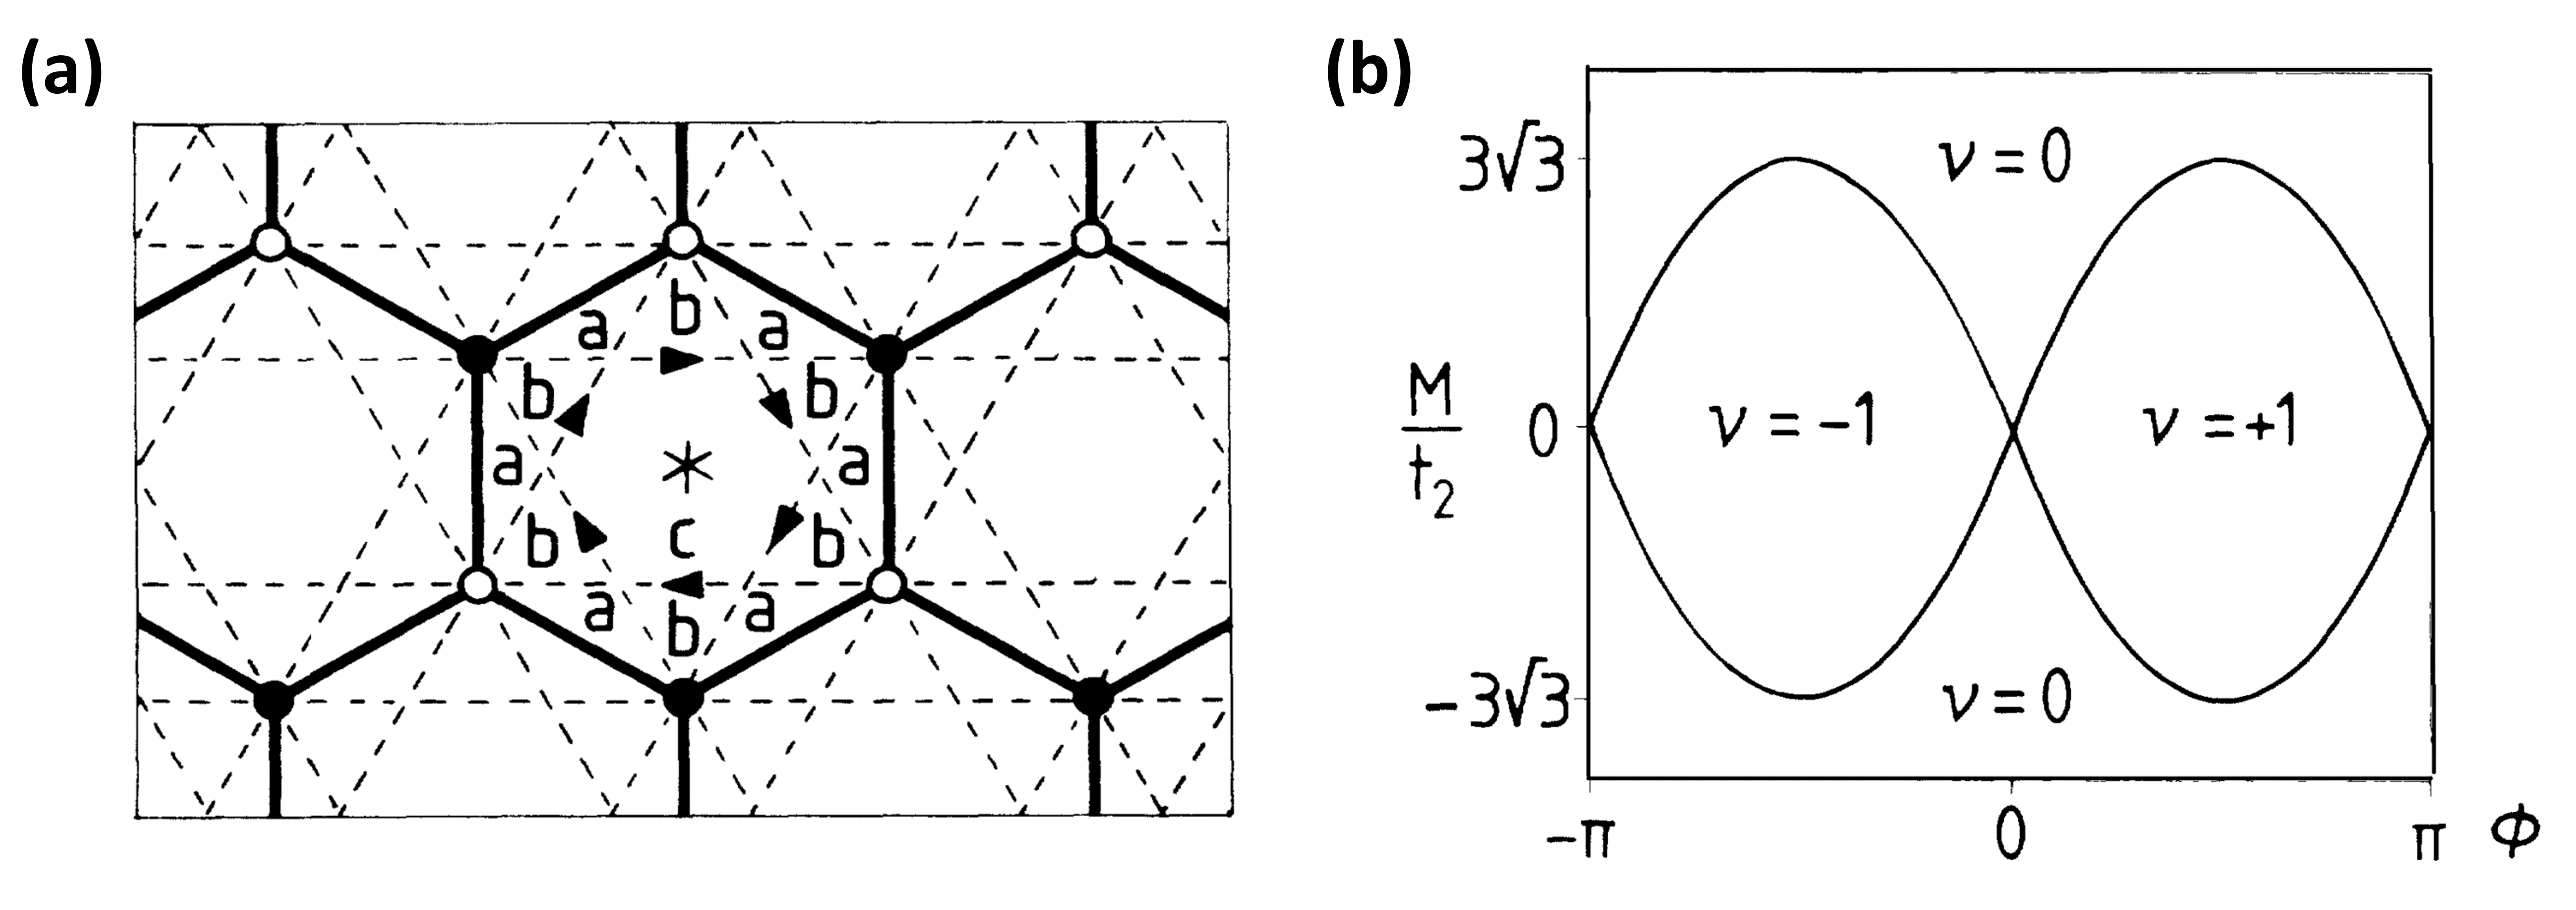
\includegraphics[width=0.75\linewidth]{figure/Introduction/HaldanePaper.png}
    \caption{霍尔丹模型的晶格与相图。 (a) 蜂窝模型示意图。实线(虚线)代表最近邻(次近邻)跃迁。空心点和实心点分别标记了A和B亚晶格的位置。次近邻跃迁的箭头标记了正相位跃迁的方向。(b) 霍尔丹模型的相图。在正弦函数$M=\pm3\sqrt{3}sin(\phi)t_2$包裹的区域内产生了非零陈数的拓扑相变$\nu=\pm1$。图片来源于文献\cite{haldane1988model}。}
    \label{fig:HaldanePaper}
\end{figure}
霍尔丹模型的k空间哈密顿量可以写作,
\begin{equation}
H(\mathbf{k}) = H_{grap}(k) + H_0(\mathbf{k}) \mathbf{I} + H_z(\mathbf{k}) \sigma_z,
\end{equation}
其中,$H_{grap}(\mathbf{k}) = t_1 \sum_i \cos(\mathbf{k} \cdot \mathbf{a}_i) \sigma_x + t_1 \sum_i \sin(\mathbf{k} \cdot \mathbf{a}_i) \sigma_y$是石墨烯哈密顿量,其在$\Gamma$点产生简并的狄拉克点(Dirac point)。单位矩阵前的部分$H_0 = 2t_2 \cos\phi \left( \sum_i \cos(\mathbf{k} \cdot \mathbf{b}_i) \right)$无法打开带隙。因此真正影响相变的项是$H_z = M - 2t_2 \sin\phi \left( \sum_i \sin(\mathbf{k} \cdot \mathbf{b}_i) \right)$,这一项会打开狄拉克点的简并。其中具有相位的次近邻项$t_2\sin\phi$打破了时间反演对称性,而位点处的势能项则打破(空间)反演对称性(inversion symmetry)。

时间反演对称性破缺导致了拓扑相变的发生。在霍尔丹模型中,系统的拓扑由陈数描述,其被定义为
\begin{equation}
    C_n = \frac{1}{2\pi} \int_{\text{BZ}} F_{n}(\mathbf{k}) \, d^2\mathbf{k}
\end{equation}
其中,$F_{n}(\mathbf{k})$是Berry曲率,它给出了 2D 表面的总量子化 Berry 通量的度量,可写作
\begin{equation}
    F_{n}(\mathbf{k}) = \nabla_{\mathbf{k}} \times \mathbf{A}_{n}(\mathbf{k})=\partial_{i} A_{j} - \partial_{j} A_{i}
\end{equation}
这里的$\partial_{i} A_{j} - \partial_{j} A_{i}$为Berry连接,其被定义为
\begin{equation}
    \mathbf{A}_{n}(\mathbf{k}) = i \langle u_{n}(\mathbf{k}) | \nabla_{\mathbf{k}} | u_{n}(\mathbf{k}) \rangle
\end{equation}
这里的$| u_{n}(\mathbf{k}) \rangle$是哈密顿量的本征态。

我们首先计算石墨烯的结果,通过精确对角化石墨烯哈密顿量,可以得到其在k空间的能带。如图\ref{fig:HaldaneBand}(a)所示,两个能带之间由简并的狄拉克点连接。计算其Berry连接,其在$K$和$K'$点都存在奇点,两个谷的Berry连接相反,因此相互抵消,这导致Berry曲率在整个平面上都为零,如图\ref{fig:HaldaneBand}(b, c)所示。一旦我们利用带有相位的次近邻项打破时间反演对称性,在图\ref{fig:HaldaneBand}(d)中,狄拉克点被打开并产生了一个带隙。此时再次计算Berry连接,可以发现仅有K谷出现奇点,这带来了一个$\nu=+1$的陈数,相应的Berry曲率也变为正值。

\begin{figure}
    \centering
    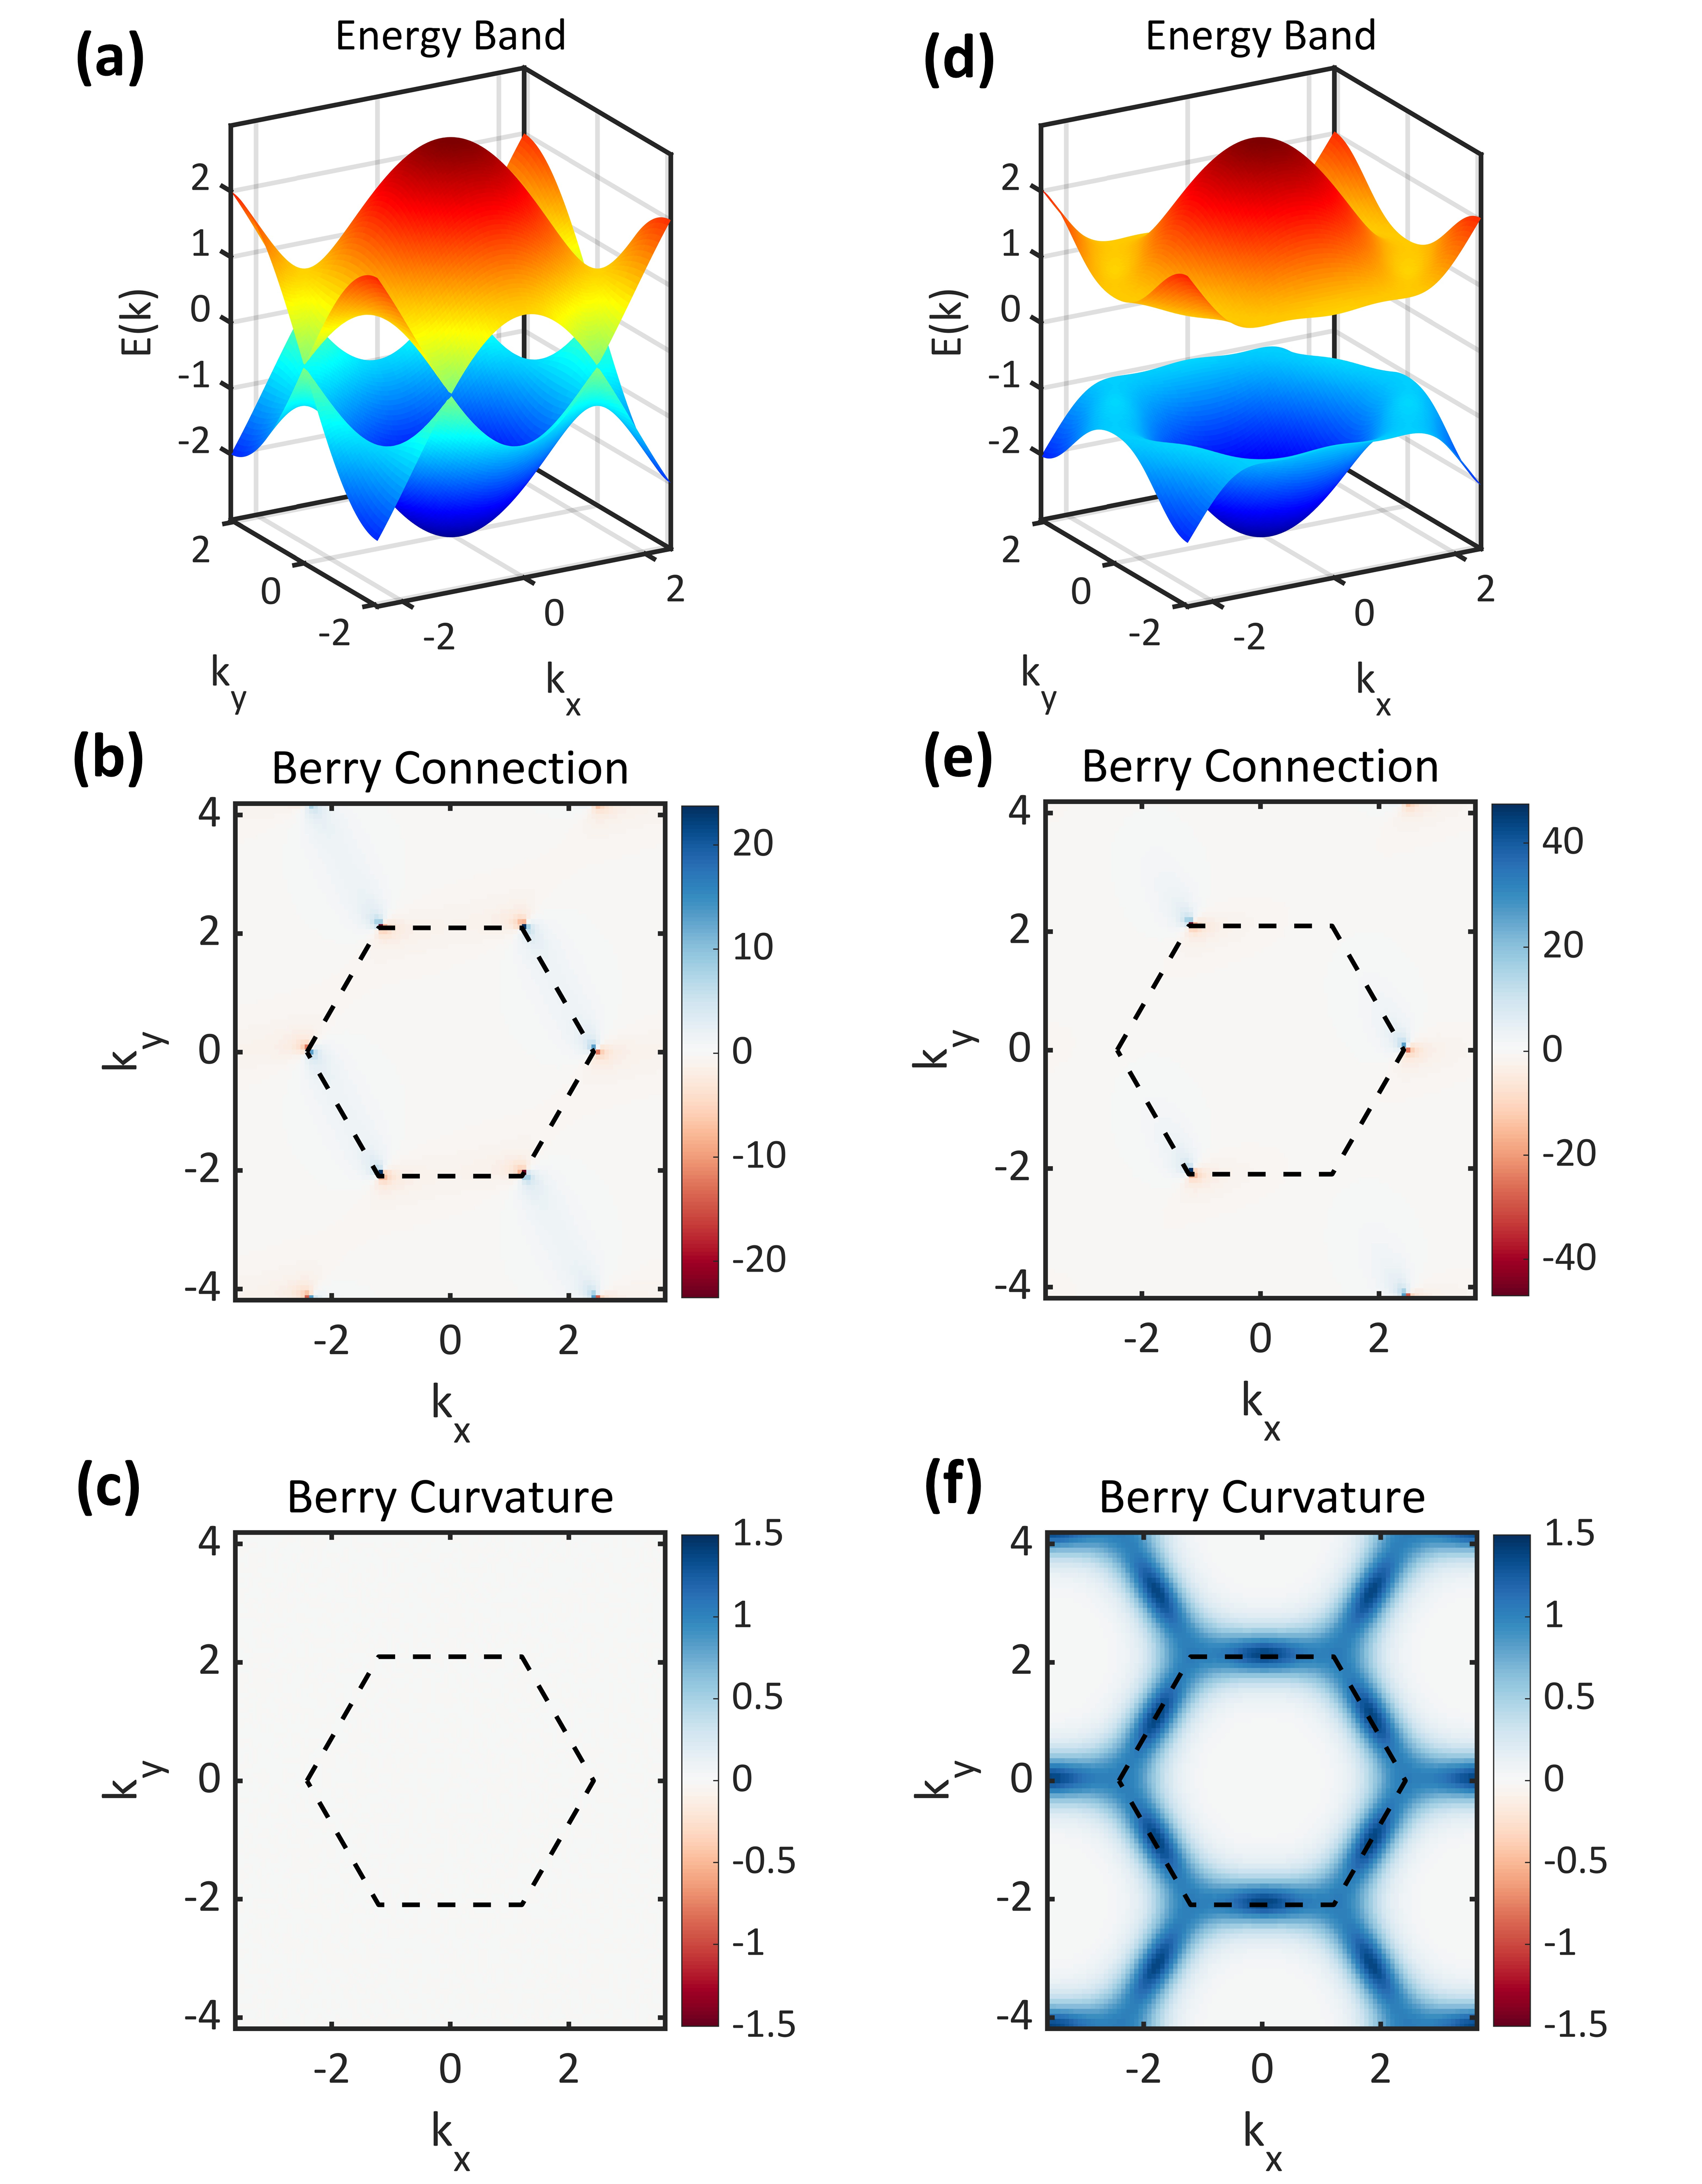
\includegraphics[width=0.65\linewidth]{figure/Introduction/HaldaneBand.png}
    \caption{(a-c) 石墨烯的能带,Berry连接和Berry曲率。(d-f) 霍尔丹模型的能带,Berry连接和Berry曲率。}
    \label{fig:HaldaneBand}
\end{figure}

当同时引入具有相位的次近邻项以及位点势能项时,时间反演对称性破缺带来的非平庸带隙和空间反演对称性带来的平庸带隙会相互竞争,最终带隙的拓扑性质取决于哪种效应更强。如图\ref{fig:HaldanePaper}(b)所示,时间反演对称性破缺带来了$\nu=\pm1$的拓扑带隙,但随着交错位势$M$的增加,原本拓扑的带隙会被闭合再打开,转化为平庸的带隙。最终两种效应的竞争形成了一个相变边界$M=\pm3\sqrt{3}sin(\phi)t_2$,如图\ref{fig:HaldanePaper}(b)所示。

量子反常霍尔效应需要交错的磁场,其实验难度高,因此直到2013年才被实验观测到\cite{chang2013experimental}。量子反常霍尔效应也被在冷原子\cite{jotzu2014experimental},光学\cite{mittal2019photonic,liu2021gain},声学\cite{li2018weyl}系统实现。量子反常霍尔效应不需要外加磁场,仅通过自发磁化实现量子霍尔效应,这是一种新的物理机制,拓宽了对霍尔效应与对称性的理解。

\subsection{分数量子霍尔效应}

在1982年,Tsui、Stormer 和 Gossard 发现了在 $1/3$ 填充处量子化霍尔电导平台\cite{PhysRevLett.48.1559},标志着分数量子霍尔效应的发现。一年后,Laughlin 给出了分数量子霍尔效应的理论解释\cite{PhysRevLett.50.1395}。Laughlin 猜测出了基态的波函数:
\begin{equation}
    \psi_{\frac{1}{m}}\left(z_i\right)=\prod_{i \neq j}\left(z_i-z_j\right)^m e^{-\frac{1}{4 l_B^2} \sum_i\left|z_i\right|^2}
\end{equation}
对于分数量子霍尔效应,处于同一个Landau 能级的电子会有强烈的库伦相互作用。库伦排斥禁止电子出现在相同的位置,因此波函数的第一项是 $z_i-z_j$,当电子 $i$ 和 $j$ 处于相同的 $z$ 时,波函数将变为零。

由于电子遵守费米统计,交换电子位置会改变波函数的符号,这要求 $m$ 必须是奇数。这也是最鲁棒的分数量子霍尔平台出现在 $1/3$ 的原因:$m=3$ 是大于 1 的第一个奇数。

假设在最低Landau 能级中有 $N$ 个粒子,Laughlin 波函数的第一项满足 $\prod_{i \neq j}\left(z_i-z_j\right)^m$。但是最低Landau 能级上的最大状态数是 $N_B$,因此填充率是 $N/N_B=1/m$。在分数填充下,每个电子会获得更多的磁通量。每个电子附着 $m$ 个磁通量。图 \ref{fig:Laughlin} 展示了 $m=3$ 的情况。

\begin{figure}[htbp]
    \centering
    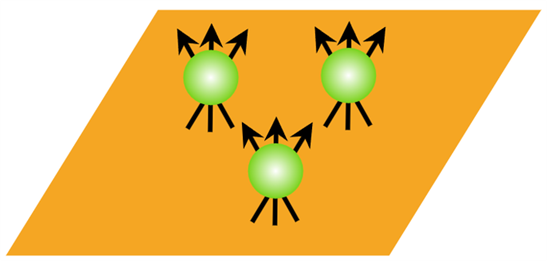
\includegraphics[width=0.35\linewidth]{figure/Introduction/Laughlin.png}
    \caption{1/3 Laughlin 波函数。}
    \label{fig:Laughlin}
\end{figure}

Laughlin 波函数解释了填充率为 $1/m$ 的一系列示例。但在 $1/m$ 外发现了更多的分数霍尔平台,如图 \ref{fig:plateau} 所示。为了解释这些新的平台,我们可以平移分数霍尔平台,将 $1/2$ 和 $0$ 磁场对齐(图 \ref{fig:plateau})。这里存在一个显著的对应关系:$1\leftrightarrow1/3$,$2\leftrightarrow2/5$,$3\leftrightarrow3/7$。因此,我们可以通过 $1, 2$ 平台来理解 $1/3, 2/5$ 平台。

\begin{figure}[htbp]
    \centering
    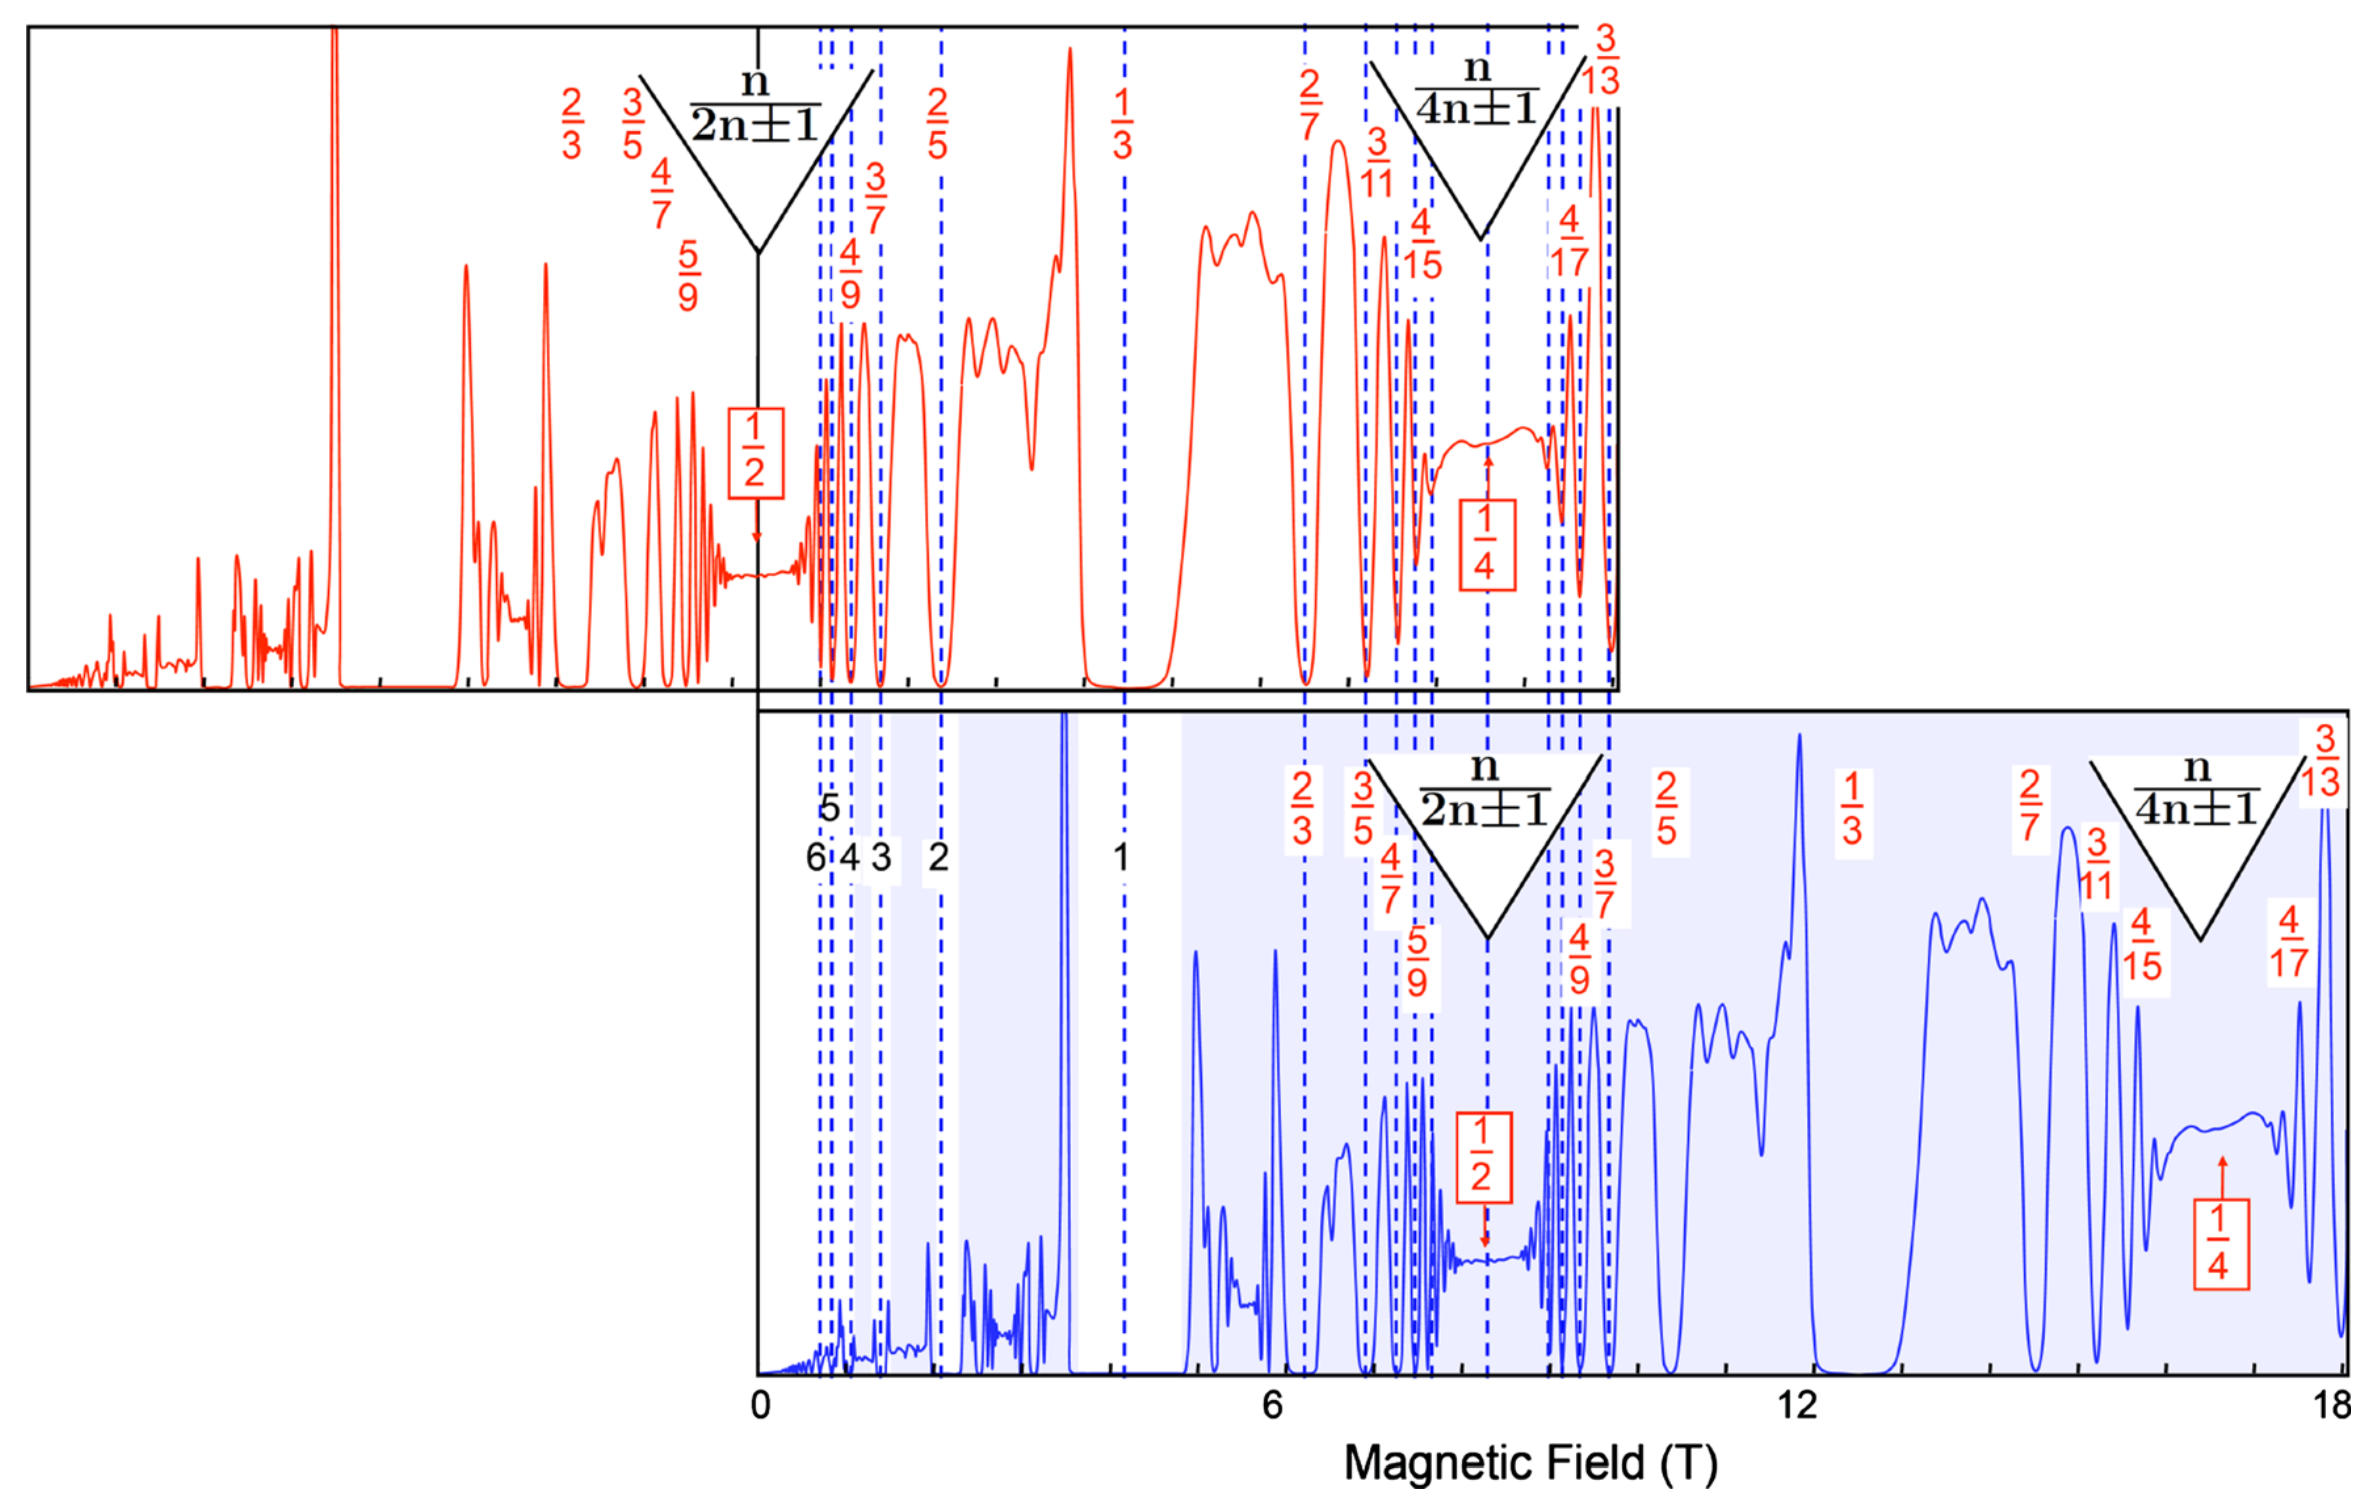
\includegraphics[width=0.8\linewidth]{figure/Introduction/plateau.png}
    \caption{分数霍尔平台的关系。图片来源于参考文献\cite{jain2014note}。}
    \label{fig:plateau}
\end{figure}

Laughlin 波函数的第一项可以重写为
\begin{equation}
    \prod_{i \neq j}\left(z_i-z_j\right)^{2s+1} = \prod_{i \neq j}\left(z_i-z_j\right)^{2s} \prod_{i \neq j}\left(z_i-z_j\right),
\end{equation}
其中第一项 $\prod_{i \neq j}\left(z_i-z_j\right)^{2s}$ 是平凡的,它不会影响费米子统计。但第二项 $\prod_{i \neq j}\left(z_i-z_j\right)$ 决定了系统是费米子统计。因此,我们可以将第一项看作电子附着了两个磁通量。附着偶数磁通量的电子被称为复合费米子(composite fermion)\cite{jain1989composite}。事实上,后一部分可以看作幂为 $1$ 的 Laughlin 波函数:
\begin{equation}
    \prod_{i \neq j}\left(z_i-z_j\right) = \prod_{i \neq j}\left(z_i-z_j\right)^{1/\nu^*},
\end{equation}
其中 $\nu^*=1$。因此 $\nu=2/5$ 平台就是复合费米子取 $s=1, \nu^*=2$ 的情况。我们可以用图 \ref{fig:CF} 来说明这一情况。
\begin{figure}[htbp]
    \centering
    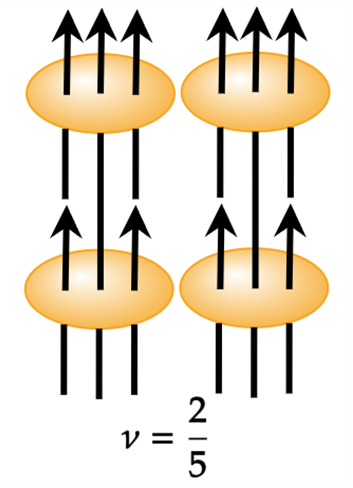
\includegraphics[width=0.25\linewidth]{figure/Introduction/CompositeFermions.png}
    \caption{2/5 复合费米子}
    \label{fig:CF}
\end{figure}

在1987年,人们观察到了一个分数填充平台 $5/2$,其分母是偶数\cite{willett1987observation}。这种现象无法用 Laughlin 波函数或复合费米子来解释。在1991年,Gregory Moore 和 Nicholas Read 提出了使用共形场论来推导分数量子霍尔系统的波函数\cite{moore1991nonabelions}。他们继续沿着 Jain 的路径,修改附加自由磁通量的形式。他们考虑了复合费米子的 $p$ 波配对,其中电子和电子形成电子对,并且对应的波函数写为 Pfaffian 形式:
\begin{equation}
    \psi_{MR}=Pf\left(\frac{1}{z_i-z_j}\right)\prod_{i \neq j}\left(z_i-z_j\right)^{2},
\end{equation}
其中 Pfaffian 是行列式的平方根,$Pf(M)=\sqrt{det(M)}$。Moore-Read 波函数除了可以解释偶数分母的一系列霍尔平台外,其另一个重要性质是它遵守非阿贝尔统计。这给实验实现非阿贝尔任意子提供了一个可能的模型。

分数量子霍尔效应带来了一种显著不同于传统能带拓扑的拓扑理论——拓扑序理论。拓扑序中的拓扑不来自于能带的开闭,而来自于相互作用粒子之间的纠缠,并表现在多体基态波函数的简并情况中。拓扑序模型的另一个重要特性是其是一个任意子模型。例如,Laughlin波函数可以产生$1/m$的分数电荷,这导致了其交换的相位不再是$\pi$的整数倍,而是一个分数,因此满足阿贝尔任意子统计。而在Moore-Read 波函数中,允许非阿贝尔任意子,是一个可能的非阿贝尔任意子的实验观测平台。拓扑序是拓扑物理的重要领域,其还有很多独特的性质被发现。但本文主旨聚焦于能带拓扑体系,因此这里只做简要介绍。

\section{高阶拓扑绝缘体}
2017年,物理学家发现了一种独特的拓扑相\cite{benalcazar2017quantized},这种拓扑相依赖于晶格内部的电子极化。在特殊的耦合条件下,电子会从平衡位置移动,形成四极矩,从而产生拓扑现象。这种特殊的拓扑相被称为高阶拓扑绝缘体(Higher-order topological insulators)\cite{schindler2018higher,xie2021higher}。高阶拓扑绝缘体的高阶体现在拓扑态和拓扑系统的维数差异上,这被称为余维数。例如量子霍尔效应,其为一个二维系统,产生了一维的边缘态,因此余维数为一。而高阶拓扑绝缘体承载着低维度、高余维度的拓扑态,譬如在二维的晶格产生零维的边界态,此时余维度为二,是一个二阶拓扑绝缘体。此外,这些高阶拓扑态局域在“边界的边界”上。对于一个一阶二维拓扑绝缘体,其开启的拓扑带隙会被一维的边界态填充。而二维二阶拓扑绝缘体,其边界哈密顿量也会打开一个带隙,由零维界面态填充。相应的,这些零维界面态也会出现在边缘态的边界处,也就是晶格的顶角,这些态被称为“角态”。

过去十年中,设计人工晶体并轻松调控耦合方案具有可行性,这些方法丰富了高阶拓扑绝缘体以及传统拓扑绝缘体的研究。迄今为止,高阶拓扑绝缘体已在经典波系统中得到广泛研究,如光子学\cite{peterson2018quantized,xie2018second,chen2019direct,xie2019visualization,mittal2019photonic,ota2019photonic,el2019corner,he2020quadrupole,zhang2020higher,li2020higher}、声学\cite{serra2018observation,zhang2019dimensional,xue2019realization,qi2020acoustic,xue2020observation,weiner2020demonstration,ni2020demonstration}和电路\cite{imhof2018topolectrical,bao2019topoelectrical,zhang2019dimensional,liu2020octupole,zhang2021experimental},并在与非厄米性\cite{luo2019higher,gao2021non}、无序\cite{zhang2021experimental,chen2020higher,li2020topological}和非线性\cite{zangeneh2019nonlinear,kirsch2021nonlinear}的相互作用中开辟了新的前沿领域。
\subsection{经典高阶拓扑模型}
二阶拓扑相指拓扑态与晶格的余维度为二的拓扑相,例如由二维晶格的零维角态或三维晶格的铰链态。最经典的二阶拓扑相是Benalcazar-Bernevig-Hughes(BBH)模型\cite{benalcazar2017quantized}。BBH模型通过调节胞内($t_1$)和胞间($t_2$)耦合强度,并引入$\pi$相流,实现了一个的四极子拓扑绝缘体(quadrapole topological insulator),如图\ref{fig:HOTIBand}(a)所示。其哈密顿量可写作
\begin{equation}
\hat{H} = \sum_\text{intra} c_i^\dagger H_\text{intra} c_i + \sum_\text{inter} c_j^\dagger H_\text{inter} c_j,
\end{equation}
其中
\begin{equation}
\begin{aligned}
H_\text{intra} = & \, t_1 (\sigma_x \otimes I + I \otimes \tau_x + \sigma_y \otimes \tau_y), \\
H_\text{inter} = & \, t_2 (\sigma_x \otimes I + I \otimes \tau_x + \sigma_y \otimes \tau_y).
\end{aligned}
\end{equation}
该模型的特点是体偶极子极化为零$p_x=p_y=0$,但具有量子化的体四极矩$Q_{xy}=1/2$。哈密顿量中的$\pi$相流使得系统打开一个带隙,如图\ref{fig:HOTIBand}(b)所示。由于扩展的高阶体-边界对应原理,二维四极子绝缘体会在带隙产生零维角态和一维边缘态。

另一种实现二阶拓扑绝缘体的经典方法是将一维SSH模型直接推广到更高维度\cite{noh2018topological,ni2019observation,zhang2019second,xue2019acoustic,zhang2020low}。此时哈密顿量的耦合矩阵可以写作
\begin{equation}
H_{\text{coup}} = \sigma_x \otimes I + I \otimes \sigma_x
\end{equation}
此时胞内耦合为$H_\text{intra}=t_1H_{\text{coup}}$,胞外耦合为$H_\text{inter}=t_2H_{\text{coup}}$,如图\ref{fig:HOTIBand}(c)所示。此时仅通过改变二维系统中胞内和胞间耦合的相对强度,无需引入$\pi$相流,也可以诱导出二阶拓扑相。但与BBH模型不同的是,其拓扑不变量是偶极子极化而非四极矩($p_x=p_y=1/2, Q_{xy}=0$)。此外,由于其能带在零能附近有分布,这导致实空间角态和体态会出现混杂[图\ref{fig:HOTIBand}(d)]。

\begin{figure}[tbp]
    \centering
    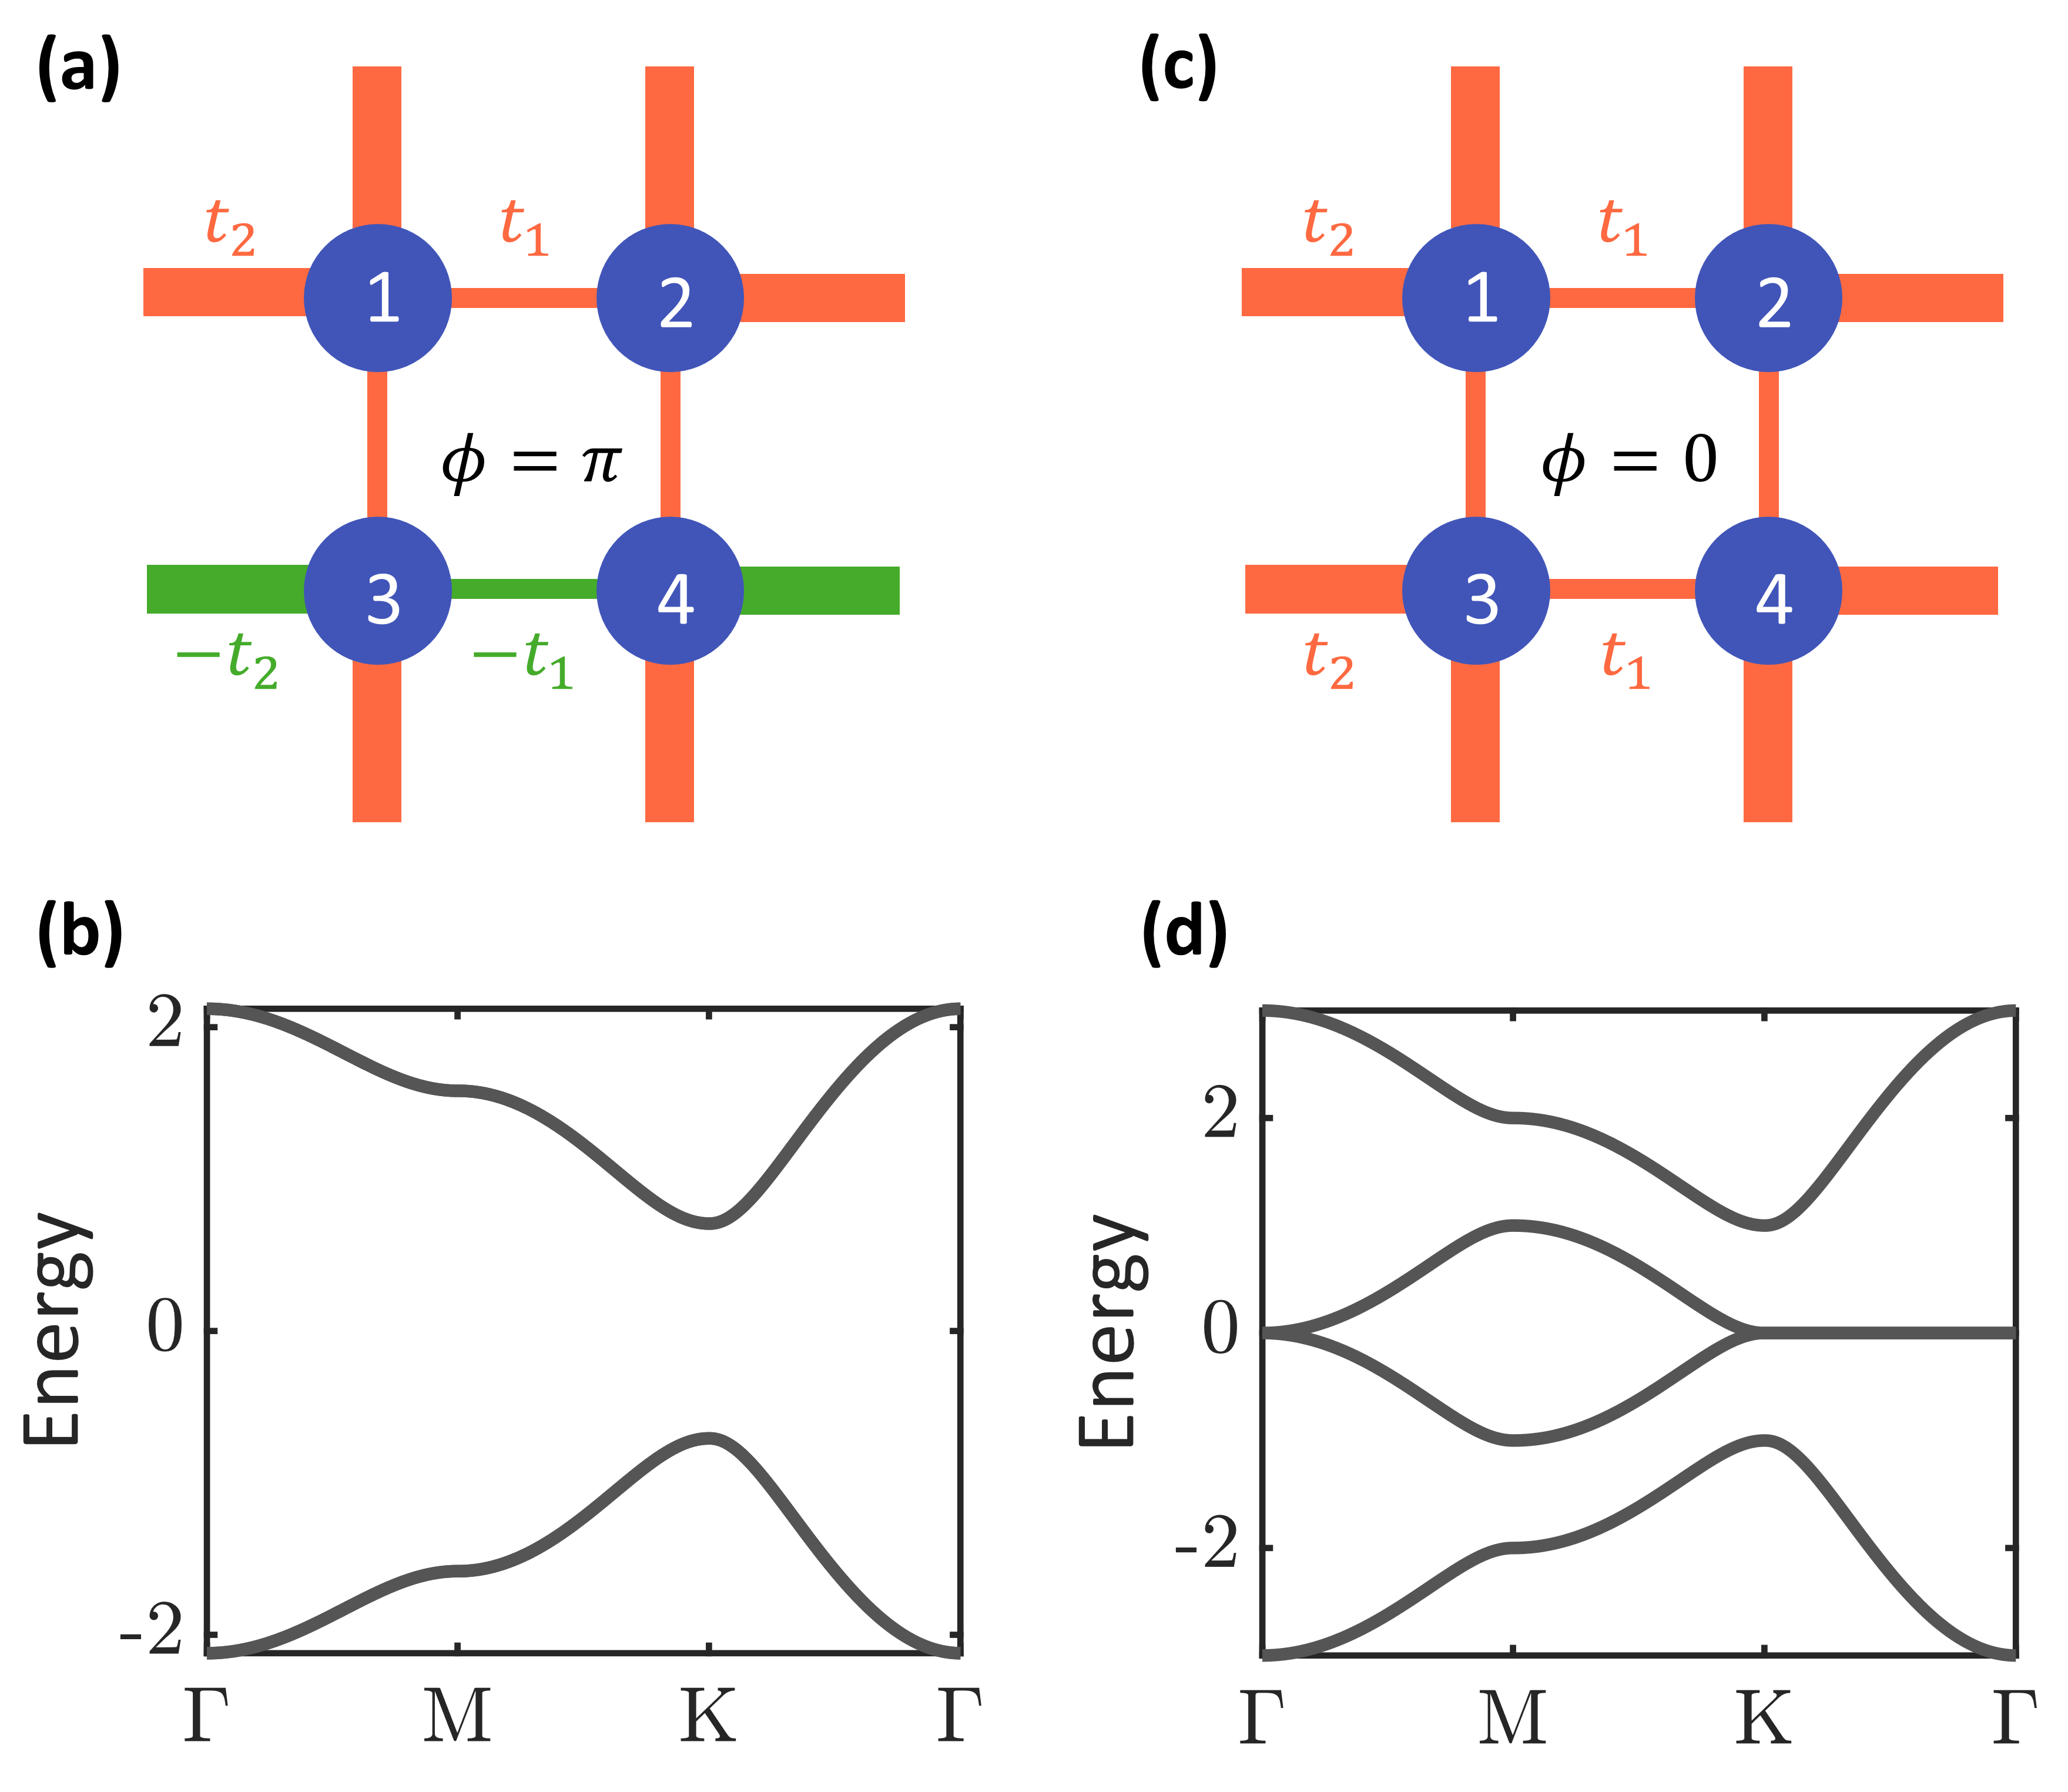
\includegraphics[width=0.5\linewidth]{figure/Introduction/HOTIBand.png}
    \caption{二阶拓扑绝缘体的耦合形式。(a) BBH模型的耦合形式。粉(绿)色代表了正(负)耦合,粗(细)线条代表胞外(胞内)耦合。由于负耦合的存在,格点围成的四方形内存在一个$\pi$相流。(b) BBH模型的能带图。(c) 二维SSH模型的耦合形式。(d) 二维SSH模型的能带图。本图选取参数$t_1=0.5, t_2=1$。}
    \label{fig:HOTIBand}
    
\end{figure}

\subsection{电荷极化与分数电荷}
高阶拓扑绝缘体的拓扑性质源于其键合-反键合的性质。交错的耦合强度使得电子倾向于向胞外某个方向移动。定向移动的电子导致晶体的电极化,形成偶极矩,四极矩和八级矩。
\begin{equation}
p_i = \int d^3r \, \rho(r) r_i, \quad 
q_{ij} = \int d^3r \, \rho(r) r_i r_j, \quad \text{and} \quad
o_{ijk} = \int d^3r \, \rho(r) r_i r_j r_k
\end{equation}
其中,$\rho(r)$是体电荷密度。图\ref{fig:polarization}展示了四极矩 (a) 和八级矩 (b) 的电荷分布。当四极矩极化的原胞堆叠为晶格时,体内沿x和y方向的电荷极化会相互抵消,因此体极化为零,但具有非零的体四极子。而当晶格有边界时,边界处的极化不会被抵消,因此有非零的边缘极化。

电荷极化的另一个结果是分数电荷\cite{benalcazar2019quantization}。高阶拓扑绝缘体属于拓扑晶体绝缘体\cite{xie2021higher,noh2018topological},因此高阶能带拓扑通过空间对称性来保护,例如反射对称\cite{langbehn2017reflection}、旋转对称\cite{schindler2018higher}、反演对称\cite{khalaf2018higher}和时间反演与旋转对称的组合\cite{geier2018second}来保护。对于一个$C_4$对称的晶格,如果产生电荷极化,如图\ref{fig:polarization}(c)所示,此时晶格电荷分布并不满足$C_4$对称。对于一个$C_4$对称性保护的拓扑相,系统势必要从体带移除在角落处极化的电子,或者在其他三个角引入三个电子到其他体带来满足对称性要求。这些“引入”或“移除”的电子会导致晶格电荷在边界处为分数。

\begin{figure}[htbp]
    \centering
    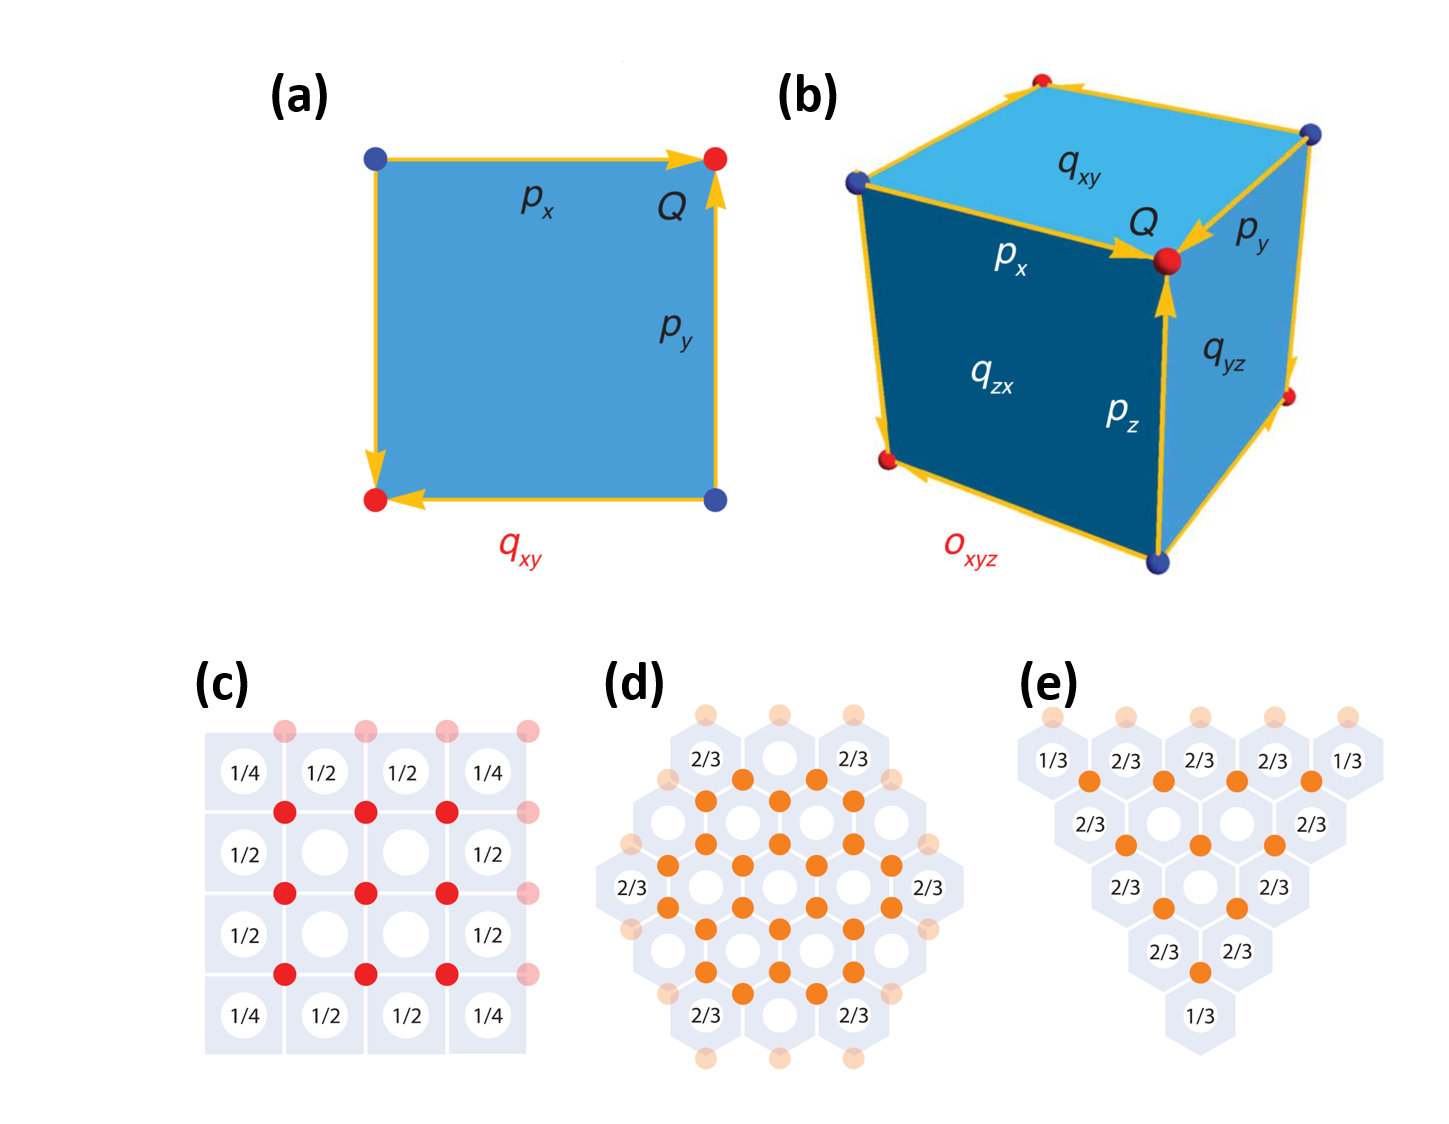
\includegraphics[width=0.75\linewidth]{figure/Introduction/polarization.png}
    \caption{电荷极化和分数电荷。(a, b)四极矩和八极矩电荷分布。(c-e) $C_4$,$C_6$和$C_3$对称晶格的电荷分布。图片来源于文献\cite{benalcazar2019quantization}。}
    \label{fig:polarization}
\end{figure}

通过对最低体带的能量进行局域态密度积分可以计算处晶格不同位置的分数电荷。以$C_4$晶格为例,电荷极化在晶格边缘产生了$1/2$的分数电荷,在晶格的角上产生了大小为$1/4$的分数电荷。类似的结果也可以在$C_6$或$C_3$对称的晶格中观测到,如图\ref{fig:polarization}(d, e)所示。对于$C_6$对称的晶格,会在晶格的角产生大小为$2/3$的分数电荷。而对于$C_3$对称的晶格,会在晶格的角产生大小为$1/3$的分数电荷。分数电荷被在电路\cite{peterson2020fractional},光学\cite{liu2021bulk}等系统实现。

\subsection{手性$Z$分类拓扑绝缘体}
在文献\cite{benalcazar2017quantized,benalcazar2019quantization}中,作者利用电荷极化来描述高阶拓扑现象,此时高阶拓扑态具有$Z_2$分类的拓扑不变量。这种拓扑来自于晶体对称性的保护,由于晶格中不均匀的电荷极化与晶格对称性的不匹配导致了局域的分数电荷。然而在上述模型中,模型遵循手性对称性,理应属于$AIII$分类。四极子绝缘体是手性耦合的堆叠一维$AIII$类拓扑绝缘体,应产生$Z$分类的拓扑不变量而不是$Z_2$分类的拓扑不变量\cite{benalcazar2022chiral}。多极矩描述将所有具有偶数绕组数的一维手性对称系统标记为平庸的。$AIII$分类预言了超过$Z_2$分类的拓扑不变量,显然需要一种不同的方法来对手性对称高阶拓扑绝缘体进行分类,即超越电荷极化到更高维度的自然推广。

在文献\cite{benalcazar2022chiral}中,作者提出了一种$Z$分类的高阶拓扑绝缘体,这种高阶拓扑绝缘体基于“多极手性数”(Multipole Chiral Numbers)这一新型的体拓扑不变量,用以描述二维和三维系统中的高阶拓扑态。多极手性数基于子晶格的多极矩算符构建,能够量化体系统边界处零能角态的数目,从而扩展了高阶拓扑物质相的分类框架。

我们从一维哈密顿量来入手,并通过一维哈密顿量的结果类比至高维来理解多极手性数的物理含义。当哈密顿量$H$具有手性,此时应满足
\begin{equation}
\tau_z H \tau_z = -H = -
\begin{pmatrix}
0 & h \\
h^\dagger & 0
\end{pmatrix}
\end{equation}
其中$\tau_z$是手性算符,哈密顿量的分块形式是手性对称系统的标准形式,表明系统可以划分为两个具有相反手性荷的子晶格$A$和$B$。

假设\(\psi_n^A\) 和 \(\psi_n^B\) 是分别位于 \( A \) 和 \( B \) 子晶格子空间中的归一化向量。在手性对称性下,每个能量为 \( \epsilon_n \) 的本征态 \( |\psi_n\rangle \) 具有一个手性伴随态:
\begin{equation}
\tau_z |\psi_n\rangle = \frac{1}{\sqrt{2}} (\psi_n^A, -\psi_n^B)^T
\end{equation}
其能量为 \( -\epsilon_n \)。对哈密顿量 \( H^2 |\psi_n\rangle = \epsilon_n^2 |\psi_n\rangle \) 的计算导致以下特征值问题:$h h^\dagger \psi_n^A = \epsilon_n^2 \psi_n^A$以及$h^\dagger h \psi_n^B = \epsilon_n^2 \psi_n^B$。因此,\(\psi_n^A\) 和 \(\psi_n^B\) 可以通过分别对 \( h h^\dagger \) 和 \( h^\dagger h \) 进行对角化来获得。

这一结构可以通过对 \( h \) 的奇异值分解(SVD)来表述:
\begin{equation}
h = U_A \Sigma U_B^\dagger
\end{equation}
其中$U_A$ 和 $U_B$ 是分别表示子晶格$A$和$B$空间的酉矩阵,$\Sigma$是对角矩阵,包含奇异值。通过这一分解,可以得到:
\begin{equation}
h h^\dagger = U_A \Sigma^2 U_A^\dagger, \quad h^\dagger h = U_B \Sigma^2 U_B^\dagger
\end{equation}
因此,\(\Sigma^2\) 中的平方奇异值对应于哈密顿量的平方能量 \( \epsilon_n^2 \)。

奇异值分解允许通过定义幺正矩阵 \( q= U_A U_B^\dagger \) 对哈密顿量进行显式展平(flattening)。此时可以定义出一维布洛赫哈密顿量(Bloch Hamiltonian)的绕数(winding number):
\begin{equation}
N_x = \frac{1}{2\pi i} \int_{\text{BZ}} \mathrm{Tr} \left[ q^\dagger(k) \partial_k q(k) \right] \, dk
\end{equation}
这是一个$Z$分类的拓扑不变量。

在不存在周期性的情况下,晶格动量 \( k \) 不再是良好的量子数,绕数的定义将失去意义。一维绕数等价于以下实空间指标:
\begin{equation}
N_x = \frac{1}{2\pi i} \mathrm{Tr} \log \left( P_x^A (P_x^B)^\dagger \right) \in \mathbb{Z}
\end{equation}
其中:
\begin{equation}
P_x^S = U_S^\dagger P_x^S U_S
\end{equation}
是偶极矩算符投影到子晶格 \( S \) 空间中的结果(\( S = A, B \))。

在此定义中,\( P_x^S \) 是基于周期性系统偶极矩算符的,但限制于单个子晶格:
\begin{equation}
P_x^S = \sum_{R, \alpha \in S} |R, \alpha \rangle \exp\left( -i \frac{2\pi R}{L} \right) \langle R, \alpha |
\end{equation}
其中\( L \)是晶格的总单元数 ,\( |R, \alpha \rangle = c_{R,\alpha}^\dagger |0\rangle \) 表示单位元 \( R \) 中轨道 \( \alpha \) 的产生算符。

这一实空间框架可以很容易的推广到更高维度。文章定义了适用于二维和三维手性对称高阶拓扑相的多极手性数。首先定义子晶格多极矩算符
\begin{equation}
\begin{aligned}
Q_{xy}^S &= \sum_{R, \alpha \in S} |R, \alpha \rangle \exp \left( -i \frac{2\pi xy}{L_x L_y} \right) \langle R, \alpha |, \\
O_{xyz}^S &= \sum_{R, \alpha \in S} |R, \alpha \rangle \exp \left( -i \frac{2\pi xyz}{L_x L_y L_z} \right) \langle R, \alpha |
\end{aligned}
\end{equation}

其中 \( R = (x, y,(z)) \) 表示晶格单元的坐标,\( L_x \)、\( L_y \) 和 \( L_z \) 是晶格在 \( x \)、\( y \) 和 \( z \) 方向上的总长度。这两个算符分别对应于四极矩和八级矩,定义在二维和三维晶格上。

此时手性二阶和三阶拓扑不变量定义为
\begin{equation}
N_{xy} = \frac{1}{2\pi i} \mathrm{Tr} \log \left( \bar{Q}_{xy}^A (\bar{Q}_{xy}^B)^\dagger \right), \\
N_{xyz} = \frac{1}{2\pi i} \mathrm{Tr} \log \left( \bar{O}_{xyz}^A (\bar{O}_{xyz}^B)^\dagger \right)
\end{equation}
这里$\bar{O}_{xy}^S = U_S^\dagger O_{xy}^SU_S$,$\bar{O}_{xyz}^S = U_S^\dagger O_{xyz}^SU_S$,其中$S=A,B$代表不同子晶格的多极矩投影。

作者实现了一个同时具有手性对称性和 \( C_4 \) 对称性,且具有长程耦合的高阶拓扑绝缘体,如图\ref{fig:CHOTI}(a)所示。在图(b)作者展示了模型的相图。在紫色区域,该系统在零能量附近具有体能隙,同时二极矩 \( q_{xy} \) 和二极手性数 \( N_{xy} \) 均表明该相是平凡相(\( q_{xy} = 0, N_{xy} = 0 \))。从这一相出发,随着 \( w_1/v \) 的增加,会发生体能隙闭合的拓扑相变,相变后系统进入非平凡相,此时 \( q_{xy} = 1/2, N_{xy} = 1 \)。当系统具有开放边界时,该相在每个角落都会出现一个零能态,这正是之前已知的四极子拓扑相。此时零能态局域在每个角落并分布于不同的子晶格,如图\ref{fig:CHOTI}(c)所示。

\begin{figure}
    \centering
    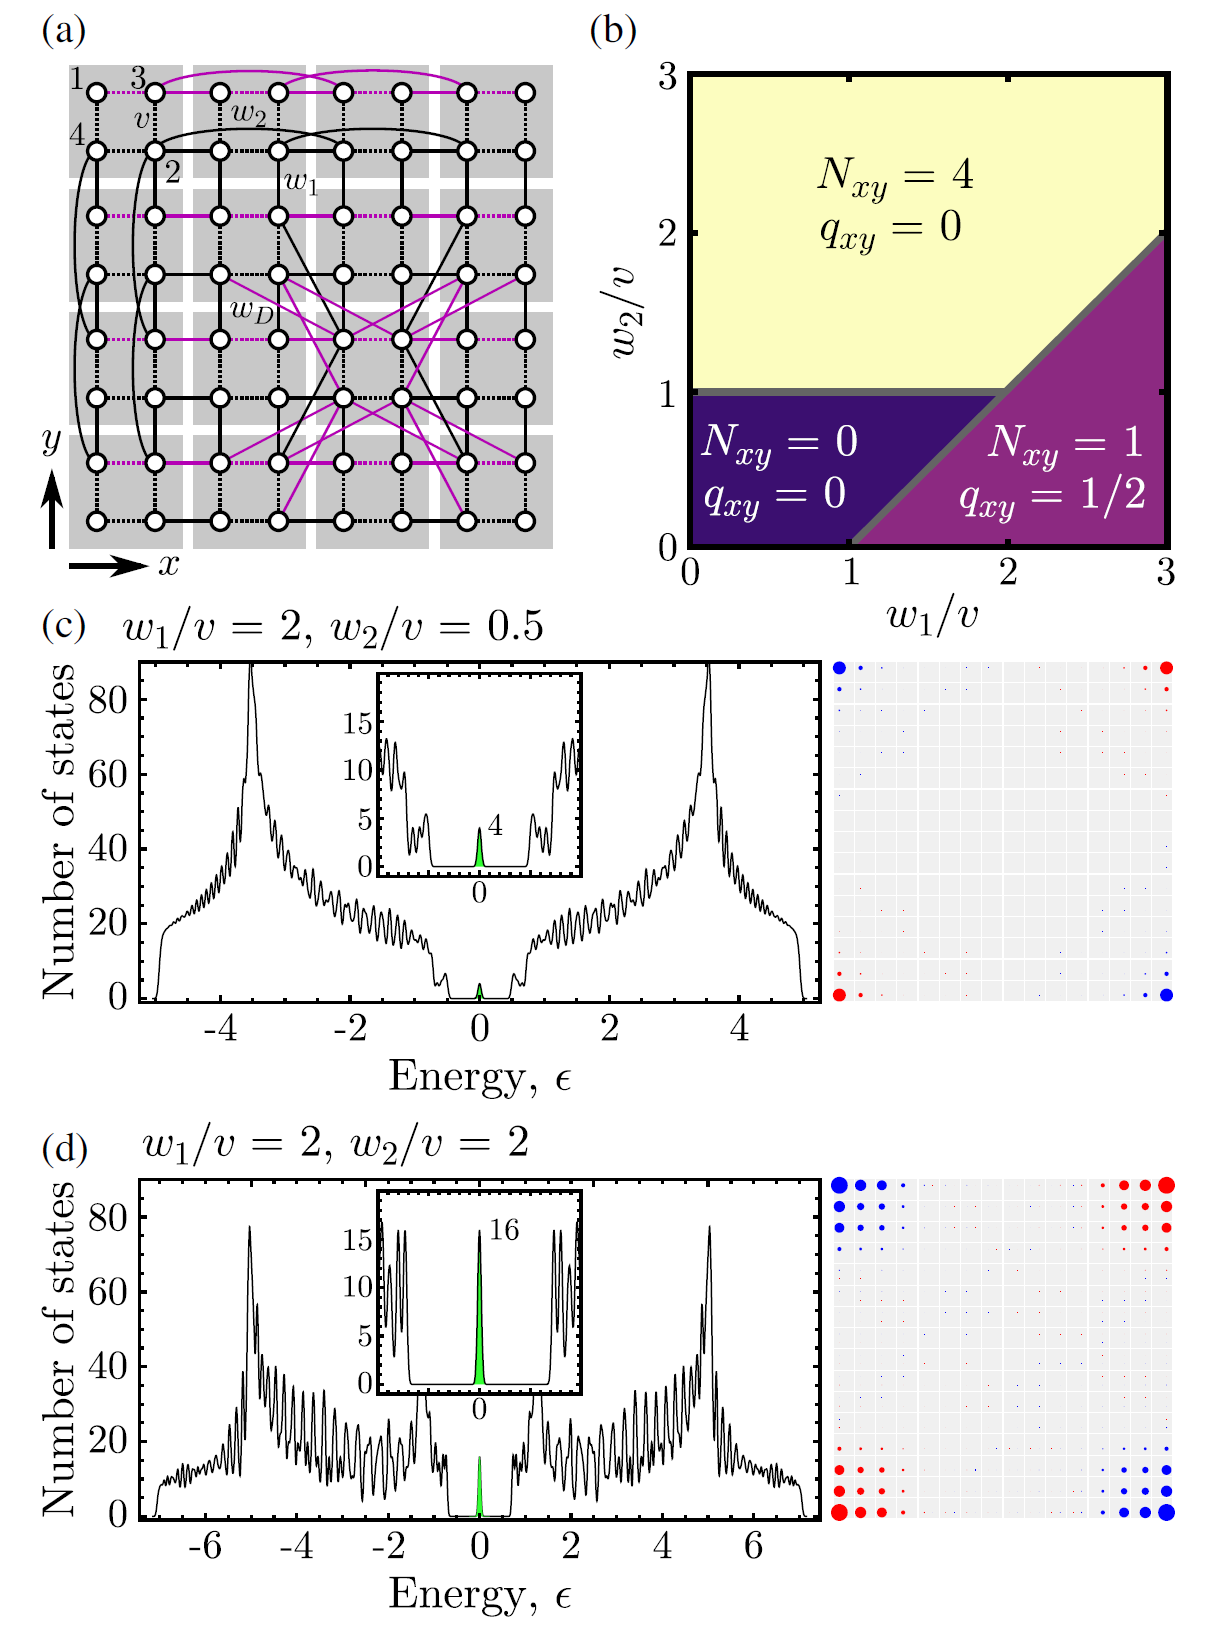
\includegraphics[width=0.5\linewidth]{figure/Introduction/CHOTI.png}
    \caption{手性$Z$分类拓扑绝缘体。(a) 手性高阶拓扑绝缘体的紧束缚模型。(b) 拓扑相图,显示了二极手性数$N_{xy}$和传统二极矩$q_{xy}$的值。(c, d) 态密度分布以及拓扑角态场分布图。其中(c)对应$N_{xy}=1$,$q_{xy}=1/2$的结果,(d)对应$N_{xy}=4$,$q_{xy}=0$的结果。图片来源于文献\cite{benalcazar2022chiral}。}
    \label{fig:CHOTI}
\end{figure}

然而,当长程跃迁 \( w_2/v \) 增加时,会发生另一个体能隙闭合的相变,分离出一个新的非平凡相 \( N_{xy} = 4 \),但此时 \( q_{xy} = 0 \)。对开放边界系统的数值模拟表明,在这一相中,每个角落处都会出现四个简并的零能态,并且所有这些零能态都集中在系统的单一子晶格上,如图\ref{fig:CHOTI}(d)所示。

与传统的Wannier中心构型或边界局域质量域机制相比,多极手性数为高阶拓扑相提供了更广泛的理解,尤其是对那些边界阻断型拓扑相的描述。这种独特的高阶拓扑绝缘体已经被实验验证\cite{li2023large,wang2023realization}。

\section{本章小结与论文的结构安排}
在本章中,我们介绍了拓扑现象的起源;接下来回顾了量子霍尔效应,反常量子霍尔效应,分数量子霍尔效应等经典的一阶拓扑模型;最后讨论了高阶拓扑相的经典模型,其拓扑性质以及近期的发展。

在本文的后续章节中,笔者将介绍分数维度的拓扑绝缘体的基础理论和最新进展。并分别在分数维度的反常量子霍尔模型和高阶拓扑模型中展开数值,仿真和实验研究。最后会对相关研究工作进行总结。具体章节安排如下:

在第二章:分形拓扑绝缘体中,笔者将详细介绍分形这一概念,以及其相应的性质,包括自相似性,分数维度的计算方法,随机分形等概念。接下来会具体介绍分形拓扑绝缘体的理论工作以及其在光学,声学以及其他系统的实验进展。

在第三章:分形霍尔丹模型理论中,笔者首先介绍了谢宾斯基三角形晶格的产生方式和晶格对应的分数维度。接下来笔者解释了分形霍尔丹模型的实现方法,其对应的哈密顿量,分形晶格实空间拓扑不变量的两种计算方法:伯特系数与实空间陈数以及它们的对比。最后笔者解释了在分形晶格下产生的拓扑相图压缩现象以及分形拓扑态的鲁棒性。

在第四章:分形霍尔丹模型的有限元仿真和实验观测中,笔者介绍了分形霍尔但模型的声学晶格等价实现。通过有限元仿真的方式,笔者仿真了霍尔丹模型的声学原胞,接着仿真了分形霍尔丹模型的频谱,确定其拓扑态频率范围。并对边缘态的特征模型,激发性质以及鲁棒性进行了仿真证明。随后笔者对声学分形霍尔丹模型进行实验验证。笔者首先介绍了实验装置以及激发探测方案。随后通过3D打印技术,笔者制备了声学分形霍尔丹模型。笔者测量了声学拓扑态,并在相图的不同区域进行测量,验证了声学分形晶格的压缩相图。

在第五章:分形BBH模型理论中,笔者首先介绍了BBH模型的哈密顿量和拓扑不变量。通过精确对角化哈密顿量,笔者计算了分形能谱和拓扑态。当胞内耦合为零时,产生了一系列单极,二聚体,三聚体以及四聚体模式。当引入胞内耦合时,出现了模式之间的混合。笔者还计算了更高迭代的晶格以证明结果的普适性。接下来笔者讨论了晶格和拓扑态的维度,笔者发现在分形晶格中,拓扑态和晶格具有相同的维度。此外,分形BBH模型也具有与分形霍尔丹模型类似的拓扑相图压缩性质。笔者计算了二维和不同迭代次数的分形晶格的拓扑相图,并解释了拓扑相图压缩的原因。最后作者计算了分形BBH模型的分数电荷,展示了分形BBH模型的鲁棒性,并提出了一个高维分形晶格的例子。

在第六章:分形BBH模型的有限元仿真和实验观测中,笔者先后介绍了分形BBH模型的有限元仿真结果和实验测量结果。笔者首先说明了在声学系统中实现等价的负耦合的方案,接着展示了声学BBH模型的原胞形式以及其动量空间频谱。最后通过求解实空间分形声学晶格的本征模式,作者得到了声学分形晶格的频谱。随后笔者者介绍了声学分形BBH模型的观测。笔者描述了具体的实验装置,并进行了实验测量方案的解释。最后作者进行了拓扑态的实验观测,并对比了实验与仿真结果。